\documentclass{article}
\usepackage{amsmath}
\usepackage{mathrsfs}
\usepackage{amssymb}
\usepackage{bbm}
\usepackage{fancyhdr}
\usepackage{graphicx}
\usepackage{subcaption}
\usepackage{natbib}
\usepackage{booktabs}
\usepackage{url}
\usepackage{hyperref}
\graphicspath{ {./Billeder/} }
\usepackage{amsthm}
\newtheorem{definition}{Definition}


\hypersetup{
    colorlinks=true,
    linkcolor=blue,       % color for internal links (sections, equations)
    citecolor=blue,       % color for citations
    urlcolor=blue         % color for URLs
}

\begin{document}
\pagenumbering{roman}
\tableofcontents
\newpage
\pagenumbering{arabic}
\section{Introduction}
When modelling prices of financial assets, modelling the volatility process itself plays a crucial role. For the price of an asset $S_t$ price dynamics are often given by a stochastic volatility model driven by a Brownian motion on the form
\begin{align}
dS_t = \mu_tS_t dt+\sigma_tS_t dB_t \label{eq:price_gen}
\end{align}
where $\mu_t$ is a drift term and $B_t$ is a one-dimensional Brownian motion. The term $\sigma_t$ represents the volatility process, and it is a very important ingredient in the model . However, modelling the volatility process itself is also a complex task. Different approaches to estimate $\sigma_t$ is used throughout the literature. In the simplest models, the volatility is either constant or a deterministic function of time but in most models the volatility process is modelled as a stochastic process itself \cite{gatheral}. \\\\
Various authors have proposed various approaches to modelling volatility. The use of fractional Brownian motions and fractional Gaussian noise in volatility modelling was in early applications such as \cite{Bollerslev} and \cite{comte} introduced to model long-range dependence in financial time series. A well-known example of such a fractional stochastic volatility model is the one proposed by \cite{comte} who models the dynamics of the volatility $\sigma_t$ of an asset as:
\begin{align*}
Y_t = \ln\sigma_t, \quad dY_t = -\gamma Y_t dt+\theta dB^H_t
\end{align*}
where $B^H$ is a fractional Brownian motion with Hurst exponent $H$. The long range dependence is modelled by choosing $1>H>\frac{1}{2}$ \cite{comte}. Fractional Brownian motions can be useful building blocks in stochastic volatility models for several reasons. Firstly, a fractional Brownian motion has the ability to model long range dependence which is measured by the slow decay $~T^{2H-2}$ of auto-correlation of functions. Secondly, it can generate trajectories of varying level of roughness (Hölder regularity) which is also governed by the Hurst exponent $H$. The long-range dependence is manifested over long time scales while roughness is manifested over short time scales. These two properties are therefore very different, and are not necessarily related. However, for a fractional Brownian motion they are linked through self-similarity and are both governed by the Hurst exponent $H$.\\\\
In more recent literature starting with \cite{gatheral}, it has been suggested to use fractional stochastic volatility models with $H<\frac{1}{2}$ for modelling volatility. Processes driven by a fractional Brownian motion with $H<\frac{1}{2}$ are referred to as 'rough processes' since these fractional Brownian motion have trajectories rougher than a standard Brownian motion. The reasoning for the choice of $H<\frac{1}{2}$ rely on empirical estimates of the roughness of realized volatility over short intraday time scales. \cite{gatheral} asses the roughness of realized volatility and find that realized volatility exhibit rough behaviour and concludes that 'volatility is rough'. Since then several rough fractional stochastic volatility models have been suggested such as the rough Heston model \cite{el2019} and the rough Bergomi model \cite{bayer2016} using a Hurst exponent $H$ near 0.1. \\\\
In practice, true spot volatility of the underlying model cannot be observed. Only realized volatility can be observed. Therefore, one cannot necessarily conclude that true spot volatility is rough just because realized volatility exhibit rough behaviour. \cite{fukasawa} and \cite{cont} show that estimation errors when estimating volatility can substantially distort the outcome of roughness estimation and lead to a downward bias in the measurement of roughness such that realized volatility appears to be rough even when instantaneous volatility is not. \\\\
To overcome this problem of "illusive roughness" caused by volatility discretization error, roughness estimators taking into account and controlling the measurement error have been introduced by \cite{han} and \cite{bolko2023}. Both of these estimators take cumulative integrated variance as input. \\\\
In this thesis, we extend the analysis from \cite{cont} and investigate further if there is statistical evidence to conclude that 'volatility is rough'. We use the roughness estimators described in both \cite{cont} and \cite{gatheral} to asses the validity of roughness estimates based on realized volatility through detailed simulation studies. Furthermore, we introduce the sequential scale roughness estimator from \cite{han} to our numerical examples which take cumulative integrated variance as input. We investigate the performance of all three estimators for measuring the roughness of sample paths of stochastic processes based on fractional Brownian motions and other stochastic processes. We then estimate the roughness from realized volatility signals and cumulative realized variance based on high-frequency observations.\\\\
Our results are broadly consistent with the findings of \cite{cont}. When using our two roughness estimators that take instantaneous or realized volatility as input, we find that even when instantaneous volatility has diffusive dynamics or is smooth (i.e. $H\geq \frac{1}{2}$) realized volatility exhibits rough behaviour corresponding to a Hurst exponent much smaller than $0.5$. In all our numerical examples realized volatility is estimated to be rough no matter what the true roughness of the underlying model is. Especially, we show that in some cases diffusive models or even smooth processes are consistent with an apparent Hurst exponent $H\simeq 0.1$ for realized volatility, similar to the values reported in empirical studies in 'rough volatility' literature. This indicates that the claim 'volatility is rough' is far from an established fact.\\\\
For the sequential scale estimator, we find that it performs well when integrated variance approximated directly from instantaneous volatility is used as input. With minor modifications, the estimator also performs reasonably well when using realized variance as input. In particular, for diffusive models, it estimates the true roughness with high accuracy. \\
However, the sequential scale estimator remains somewhat susceptible to estimation errors in the cumulative integrated variance. Although this estimation error is small, it is sufficient to distort the outcome of the roughness estimation. Specifically, for smooth processes (i.e., $H > \frac{1}{2}$), the roughness estimates derived from realized variance are often near $0.5$, suggesting diffusive behaviour. Similarly, rough processes are estimated to be closer to diffusive behaviour (i.e., $H = \frac{1}{2}$) than they actually are. \\
Thus, while we do not observe 'illusory roughness' in realized data when using the sequential scale estimator, it does not fully mitigate the distortion caused by estimation errors.

\section{Fractional Brownian motion}
Fractional Brownian motions work well as building blocks for stochastic volatility models. In this section, we will define the fractional Brownian motion, and briefly discuss some of fBm's most important properties. The definitions and properties will mainly follow the theory in \cite{biagini2008}.\\\\ 
A fractional Brownian motion (fBm for short) $(B_t^H)_{t\in\mathbb{R}}$ with Hurst parameter $H\in(0,1)$ is a centered continuous Gaussian process with covariance function
\begin{align}
\mathbb{E}\left[B_t^HB_s^H\right] = \frac{1}{2}\left(t^{2H}+S^{2H}-\vert t-s\vert ^{2H} \right) \label{eq:fbm}
\end{align}
for $s,t\geq 0$. For $H = \frac{1}{2}$ the fractional Brownian motion reduces to an ordinary Brownian motion. The incremental process of a fractional Brownian motion is called fractional Gaussian noise.\\
From \eqref{eq:fbm} it can be seen that a fractional Brownian motion has the following properties:
\begin{enumerate}
    \item $B_0^H = 0$ and $\mathbb{E}[B^H_t] = 0$ for all $t\geq 0$.
    \item $B^H$ has homogeneous increments i.e. $B^H_{t+s}-B^H_s$ has the same law of $B^H_t$ for $s,t\geq0$.
    \item $B^H$ is a Gaussian process and $\mathbb{E}[(B^H_t)^2]=t^{2H}$, $t\geq 0$ for all $H\in (0,1)$.
    \item $B^H$ has continuous trajectories.
\end{enumerate}
The fractional Brownian motion can be divided into three very different families corresponding to $0<H<\frac{1}{2}$, $H=\frac{1}{2}$ and $\frac{1}{2}<H<1$. Looking at the correlation between two increments, we have that for $H=\frac{1}{2}$ the increments are independent since it is a Brownian motion. For $H\neq \frac{1}{2}$ the increments are not independent. From \eqref{eq:fbm} it can be seen that the covariance between the increments $B^H_{t+h}-B^H_{t}$ and $B^H_{s+h}-B^H_{s}$ with $s+h\leq t$ and $t-s=nh$ is
\begin{align*}
\rho_H(n) = \frac{1}{2}h^{2H} \left( (n+1)^{2H} +(n-1)^{2H} -2n^{2H}\right).
\end{align*}
In particular, we have for $n=1$ meaning two increments of the form $B^H_{t+h}-B^H_{t}$ and $B^H_{t+2h}-B^H_{t+h}$ that the increments are positively correlated for $H>\frac{1}{2}$ and negatively correlated for $H<\frac{1}{2}$.\\
When $h=1$ meaning that the incremental process has time step 1 we have that
\begin{align*}
\rho_H(n) = \frac{1}{2}\left( (n+1)^{2H} +(n-1)^{2H} -2n^{2H}\right) \sim H(2H-1)n^{2H-2}
\end{align*}
as $n\rightarrow \infty$. Thus, we see that $\sum_{n=1}^\infty \rho_H(n) =\infty$ for $H>\frac{1}{2}$ and $\sum_{n=1}^\infty \lvert \rho_H(n) \rvert <\infty$ for $H<\frac{1}{2}$. The non-summable autocovariance function in the case $H>\frac{1}{2}$ is equivalent to long-range dependence and it indicates slow decay of the covariance function. That is, for $H>\frac{1}{2}$ the fBm has long-range dependence but for $H<\frac{1}{2}$ it does not. \\\\
Furthermore, we have that the covariance function of the fBm is homogeneous of order $2H$. That is, 
\begin{align*}
\mathbb{E}\left[B_{at}^HB_{as}^H\right] = a^{2H} \mathbb{E}\left[B_t^HB_s^H\right].
\end{align*}
That implies that $B_{at}^H$ has the same distribution law as $a^{-H}B_t^H$ for all $H\in (0,1)$. This is known as statistical self-similarity with Hurst index $H$.\\\\
Furthermore, it can be shown that $B_t^H$ is almost surely Hölder continuous of order $\alpha$ for any $\alpha < H$. Hölder continuity is also known as Hölder regularity or simply as the roughness or smoothness of a sample path. Therefore, the roughness of $B_t^H$ completely follows the Hurst exponent $H$. Thus, we have that a fractional Brownian motion with Hurst exponent $\frac{1}{2}<H<1$ has long range dependence in increments and trajectories smoother than a Brownian motion while for $0<H<\frac{1}{2}$ the fBm has negatively correlated increments (without long range dependence) and trajectories rougher than a Brownian motion \cite{biagini2008}.\\\\
In this thesis, we will be simulating high-frequency data based on fractional Brownian motions when performing numerical experiments. Exact simulation of a fractional Brownian motion is computationally challenging, and we will in this thesis simulate paths from the fBm by using a spectral method. More details on this method is described in Appendix \ref{sec:sim_fbm}.

\section{Estimating the roughness of volatility}
Measuring the roughness of volatility is in practice not an easy task. 
In practice, we observe only a singe price path with discrete observation times, and we need to determine the roughness of this path sampled at high frequency. In order to design proper estimators it is crucial to be able to determine the roughness of realized volatility, and multiple ways of measuring the roughness exist in literature. In this section we will introduce three different roughness estimators and the theory behind them. Firstly, we will be using the roughness index estimator via $p$-th variation $\widehat{H}_{L,K}$ which was first introduced by \cite{cont}. Secondly, we will describe the roughness estimator via log regression $\widehat{H}_{R}$ introduced by \cite{gatheral}. Thirdly, we will be using the sequential scale estimator $\widehat{\mathscr{R}}_n^s$ originally developed by \cite{han}. The explained theory and rationale behind the estimators will closely follow the theory from the original articles. In Section \ref{sec:num_exp} we will conduct numerical experiments, and we will compare the performance of the three roughness estimators. 
\subsection{Instantaneous volatility and realized volatility}
Before we introduce the details of our roughness estimators we will start by explaining the concepts of instantaneous volatility and realized volatility. As mentioned in \eqref{eq:price_gen} price dynamics are often modelled on the form
\begin{align*}
dS_t = \mu_tS_t dt+\sigma_tS_t dB_t.
\end{align*}
The term $\sigma_t$ represents the volatility process, and $\sigma_t$ is also called instantaneous volatility or spot volatility. Thus, instantaneous volatility $\sigma_t$ is the true volatility of the underlying model. In stochastic volatility models, $\sigma_t$ is represented as a stochastic process itself often driven by a Brownian motion or a fractional process. Contrary to prices of an asset, instantaneous volatility cannot be directly observed and needs to be estimated from prices.\\\\
In a practical situation, the price of the asset $S_t$ at time $t$ is usually observed over a non-uniform time grid of $[0,T]$:
\begin{align*}
\pi^n = \left(0=t^n_0<t^n_1<...<t^n_{N(\pi^n)}=T\right)
\end{align*}
where $n$ is the sample frequency and $N(\pi^n)$ denotes the number of intervals in the partition $\pi^n$. In order to study high-frequency asymptotics of roughness estimators, it is often assumed that
\begin{align}
\lvert \pi^n \rvert := \sup_{i=1, \dots, N(\pi^n)} \lvert t_i^n - t_{i-1}^n \rvert  {\overset{n \to \infty}{\longrightarrow}} 0. \label{eq:time_assumption}
\end{align}
That is, the size of the largest interval of $\pi^n$ will converge to 0 as $n\rightarrow \infty$ where $n$ can be thought of as a sampling frequency i.e. the number of samples per second (or per other unit).\\\\
Instantaneous volatility $\sigma_t$ can then be recovered from integrated variance or quadratic variation of log-prices $\log S$ along this time grid by
\begin{align*}
\sigma_t^2 =  \frac{d}{dt} [\log S]_\pi (t)
\end{align*} 
where the quadratic variation of the log-price $[\log S]_\pi (t)$ is defined as 
\begin{align*}
[\log S]_\pi (t) = \lim_{n\rightarrow \infty} \sum_{\pi^n \cap [0,t]} \left( \log \frac{S(t^n_{i+1})}{S(t^n_i)}\right)^2 = \lim_{n\rightarrow \infty} RV_t^2(\pi^n)^2
\end{align*}
where $RV_t^2(\pi^n)^2$ is realized variance along the sampling grid $\pi^n$. Hence, $\sigma_t$ can be recovered from a high-frequency limit of realized variance where the realized variance along the sampling grid $\pi_n$, $RV_t^2(\pi^n)^2$, is defined as
\begin{align*}
RV_t(\pi^n)^2 = \sum_{\pi^n \cap [0,t]}\left(\log \frac{S(t^n_{i+1})}{S(t^n_i)}\right)^2.
\end{align*} 
We then simply define realized volatility as the square root of realized variance. This leads to the following formal definition: 
\begin{definition}
Realized volatility of a price process $S$ over the time interval $[t,t+\Delta]$ along the sampling grid $\pi^n$ is defined as 
\begin{align*}
RV_{t,t+\Delta}(\pi^n) = \sqrt{\sum_{\pi^n \cap [t,t+\Delta]}\left(\log \frac{S(t^n_{i+1})}{S(t^n_i)}\right)^2}. 
\end{align*}
\label{def:real_vol}
\end{definition}
If the price $S_t$ is a continuous semimartingale then the quadratic variation equals the integrated variance of $\log S$ which is given by
\begin{align*}
\left\langle log S \right\rangle = \int_0^t \sigma_s^2 ds.
\end{align*}
Furthermore, if $S_t$ follows a stochastic volatility model given by price dynamics as in \eqref{eq:price_gen}, it is known that the realized variance converges in probability to the integrated variance of $\log S$ as sampling frequency increases \cite{jacod2012}. That is,
\begin{align*}
RV_t^2(\pi^n)^2 (\pi^n) \overset{\mathbb{P}}{\underset{n \to \infty}{\longrightarrow}} \int_0^t \sigma_s^2 ds.
\end{align*} 
From that we immediately obtain that realized volatility converges to
\begin{align*}
 RV_{t,t+\Delta} (\pi^n) \overset{\mathbb{P}}{\underset{n \to \infty}{\longrightarrow}} \sqrt{\int^{t+\Delta}_t\sigma^2_s ds}.
\end{align*}
Hence, along a single price path observed at high-frequency, we can compute the realized volatility as in Definition \ref{def:real_vol} and use this as an indicator of volatility
\begin{align*}
 RV_{t,t+\Delta} (\pi^n)\simeq \sqrt{\Delta} \sigma_t.
\end{align*}
More precisely, rescaled realized volatility $\frac{1}{\sqrt{\Delta}}RV_{t,t+\Delta}$ can be used as proxy values $\hat{\sigma}_t$ of instantaneous volatility $\sigma_t$. As $n$ increases the estimation becomes more accurate \cite{cont}.\\\\
Several empirical studies including \cite{gatheral} have attempted to estimate roughness of volatility by estimating the roughness of realized volatility signals (i.e. proxy values $\hat{\sigma}_t$) using high-frequency data. Since carried out on high-frequency data, it is then assumed that the difference between $\hat{\sigma}_t$ and $\sigma_t$ is relatively small, and that the estimated roughness of realized volatility signals also works as a good estimation of the roughness of the instantaneous volatility process $\sigma_t$. However, there is no guarantee that $\hat{\sigma}_t$ and $\sigma_t$ exhibits same kind of roughness behaviour, and as we will illustrate later on estimation error in proxy values $\hat{\sigma}_t$ can substantially distort the roughness estimation.

\subsection{Roughness index estimator via $p$-th variation}
In this section, we will describe the roughness index estimator via normalized $p$-th variation which was introduced in \cite{cont}. We will closely follow the theory and methodology behind the estimator described in \cite{cont}.\\\\
We are working with partitions of our time interval. Consider a sequence of partitions $\pi = (\pi^n) _{n\geq 1}$ of $[0,T]$ where
\[
\pi^n = \left( 0 = t_0^n < t_1^n < ... < t^n_{N(\pi^n)}=T \right)
\]
represents observation times at frequency $n$. We again let $N(\pi^n)$ denotes the number of intervals in the partition $\pi^n$. We assume that assumption \eqref{eq:time_assumption} is fulfilled for all time partitions considered. That is, the size of the largest interval of $\pi^n$ will converge to 0 as the sampling frequency increases $n\rightarrow \infty$.\\\\
We will now define the concept of $p$-th variation along a sequence of partitions $(\pi^n) _{n\geq 1}$:
\begin{definition}
\textnormal{(p-th variation along a sequence of partitions)}\\
$x \in C^0([0,T], \mathbb{R})$ has finite p-th variation along the sequence of partitions 
$\pi = (\pi^n, n \geq 1)$ if there exists a continuous increasing function $[x]_{\pi}^{(p)}: [0,T] \to \mathbb{R}_+$ such that
\begin{align}
\forall t \in [0,T], \quad \sum_{\{t_j^n, t_{j+1}^n\} \in \pi^n: t_j^n \leq t} \lvert x(t_{j+1}^n) - x(t_j^n) \rvert^p 
{\overset{n \to \infty}\longrightarrow} [x]_{\pi}^{(p)}(t). \label{eq:pth_def}
\end{align}
If this property holds, then the convergence in \eqref{eq:pth_def} is uniform. We call $[x]_{\pi}^{(p)}$ the p-th variation of $x$ along the sequence of partitions $\pi$. We denote $V_\pi^p([0,T], \mathbb{R})$ the set of all continuous paths with finite p-th variation along $\pi$.
\label{def:pth_var}
\end{definition}
The concept of roughness will then be formalized using the notion of variation index and roughness index.
\begin{definition}
\textnormal{(Variation index)}\\
The variation index of a path $x$ along a partition sequence $\pi$ is defined as the smallest $p \geq 1$ for which $x$ has finite p-th variation along $\pi$:
\begin{align*}
p^{\pi}(x) = \inf \left\{ p \geq 1 : x \in V_{\pi}^p([0,T], \mathbb{R}) \right\}.
\end{align*}
\label{def:var_index}
\end{definition}
\begin{definition}
\textnormal{(Roughness index)}\\
The roughness index of a path $x$ (along $\pi$) is defined as
\begin{align*}
H^{\pi}(x) = \frac{1}{p^{\pi}(x)}.
\end{align*}
\label{def:rough_index}
\end{definition}
When the underlying sequence of partitions is clear, we will simply denote these indexes as $p(x)$ and $H(x)$. \\\\
For a real-valued stochastic process $X: [0,T]\times \Omega \rightarrow \mathbb{R}$ the variation index $p^\pi (X(.,\omega))$ of each sample path $X(.,\omega)$ may in principle be different. However, there are many important classes of stochastic processes which have an almost-sure roughness index. For example we have that along the dyadic partition sequence 
\begin{align}
\pi^n = \left( t_i^n = \frac{iT}{2^n}, i=0,1,...,2^n \right), \label{eq:dya_part}
\end{align}
the fractional Brownian motion $B_t^H$ has roughness index $H^\pi(x) = H$  matching the Hurst exponent $H$ and the Hölder regularity \cite{cont}.\\
However, existence of variation index is in general not obvious. Further details can be seen in \cite{han2022hurst}.\\\\
When estimating roughness from empirical data based on discrete observations, using the $p$-th variation directly is difficult since it involves checking convergence to an unknown limit. To this end, \cite{cont} introduce the concept of normalized $p$-th variation which has better asymptotics:
\begin{definition}
\textnormal{(Normalized p-th variation along a sequence of partitions)}\\
Let $\pi$ be a sequence of partitions of $[0, T]$ with mesh $\lvert \pi^n \rvert \to 0$ and 
$\pi^n = \{ 0 = t_1^n < t_2^n < \cdots < t_{N(\pi^n)}^n = T \}$. 
$x \in V_{\pi}^p([0, T], \mathbb{R})$ is said to have normalized p-th variation along $\pi$ 
if there exists a continuous function $w(x, p, \pi) : [0, T] \to \mathbb{R}$ such that:
\begin{align*}
\forall t \in [0, T], \quad \sum_{\pi^n \cap [0,t]} \lvert x(t_{j+1}^n) - x(t_j^n) \rvert^p \to w(x, p, \pi)(t).
\end{align*}
\label{def:norm_pth_var}
\end{definition}
\cite{cont} justify the terminology by a result that shows that for a large class of functions with $p$-th variation, the normalized $p$-th variation exists and is linear. Furthermore, it can be shown that the normalized $p$-th variation is a 'sharp' statistic meaning that if a function has finite $p$-th variation then for all $q\neq p$ the normalized $p$-th variation is either zero or infinite. Additionally, it is shown that a fractional Brownian motion has normalized $p$-th variation along the dyadic partition $\pi^n$ as in \eqref{eq:dya_part} almost-surely.
\subsubsection{Estimating the roughness from discrete observations}
With these concepts defined we now proceed to explaining how roughness can be estimated from discrete observations. Given discrete observations on a refining partition $\pi^L$ we define the 'normalized $p$-th variation statistic' which is the discrete counterpart of the normalized $p$-th variation as
\begin{align}
W(L, K, \pi, p, t, X) := \sum_{\pi^K\cap [0,t] } \frac{\lvert X(t_{i+1}^K)-X(t_i^K)\rvert^p}{\sum_{\pi^L\cap [t_i^K, t_{i+1}^K]}\lvert X(t_{j+1}^L)-X(t_j^L)\rvert^p} \times (t_{i+1}^K-t_i^K). \label{eq:w_stat_def}
\end{align}
This definition involves two frequencies $K$ and $L>>K$. We can consider $L$ as the sample frequency while $K$ is a block frequency such that $\pi^K$ is a subpartition of $\pi^L$. Thus, we are grouping the sample size $L$ into $K$ many groups where each group contains exactly $\frac{L}{K}$ consecutive points. It can be seen that the normalized $p$-th variation statistic converges to the normalized $p$-th variation as $L$ and $K$ increase. That is,
\begin{align*}
\lim_{K\rightarrow\infty}\lim_{L\rightarrow\infty} W(L, K, \pi, p, t, X) = w(x, p, \pi)(t).
\end{align*}
The variation index estimator $\hat{p}^\pi_{L,K}(X)$ associated with data sampled on $\pi^L$ can then be obtained by computing $W(L, K, \pi, p, t, X)$ for different values of $p$ such that the following equation can be solved for $p^\pi_{L,K}(X)$
\begin{align}
W(L, K, \pi, \hat{p}^\pi_{L,K}(X), t, X) = T. \label{eq:wpth}
\end{align}
The corresponding roughness index estimator is then defined as
\begin{align*}
\hat{H}^\pi_{L,K}(X) = \frac{1}{\hat{p}^\pi_{L,K}(X)}.
\end{align*}
If the underlying dataset and partition is clear we will also denote this estimator simply as $\widehat{H}_{L,K}$. We will refer to $\widehat{H}_{L,K}$ as the roughness index estimator via $p$-th variation. 
\subsubsection{Sample behaviour of $\widehat{H}_{L,K}$}
We will now study the behaviour of the roughness estimator based on high-frequency simulated data. We will be simulating from a fractional Brownian motion $B_t^H$ where the true roughness is known to be $H$. For the simulated paths we then compute the roughness index estimator via $p$-th variation $\widehat{H}_{L,K}$ and investigate its performance. We will in these examples be using a uniform partition of the time interval $[0,1]$ with
\begin{align*}
\pi^n = \left( 0 < \frac{1}{n}< \frac{2}{n}<...< 1\right).
\end{align*}
We generate data from four fractional Brownian motions with different Hurst exponents $H=\{0.1,0.3,0.5,0.8\}$. For every simulated path we compute the statistic $W(L=300\times 300, K=300, \pi, p, t=1, X=B^H)$ for different values of $p$. Thus, we use $\pi^L$ as our partition of time and generate $L=300\times 300$ points uniformly on the interval $[0,1]$.\\
The roughness estimator $\widehat{H}_{L,K}$ solves equation \eqref{eq:wpth} with $T=1$. To visualize this we plot $\log(W(L=300\times 300, K=300, \pi, p, t=1, X=B^H))$ against $H=1/p$. The results are presented in Figure \ref{fig:checkw}. The solid black line is the value of $\log(W(L=300\times 300, K=300, \pi, p, t=1, X=B^H))$ for different values of $1/p$. The blue vertical line represents the estimated roughness index whereas the black dotted vertical line represent the true Hurst parameter of the underlying model. The blue horizontal line represents $W(L, K, \pi, p, t, X) = 1$ which is the equation $\widehat{H}_{L,K}$ solves. Thus, the estimated roughness index $\widehat{H}_{L,K}$ is found in the crossing between $\log(W(L=300\times 300, K=300, \pi, p, t=1, X=B^H))$ (solid black line) and $W(L, K, \pi, p, t, X) = 1$ (blue horizontal line).
\begin{figure}[htbp]
    \centering
    
    \begin{subfigure}{0.48\textwidth}
        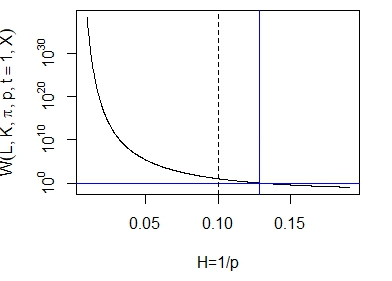
\includegraphics[width=\linewidth]{wagainstp_H01.png}
    \end{subfigure}
    \hfill
    \begin{subfigure}{0.48\textwidth}
        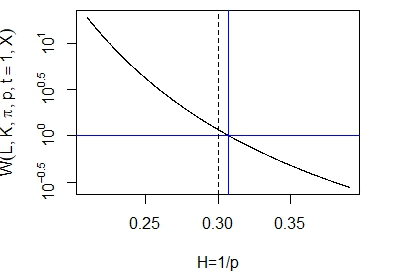
\includegraphics[width=\linewidth]{wagainstp_H03.png}
    \end{subfigure}
    \vskip 0em
    \begin{subfigure}{0.48\textwidth}
        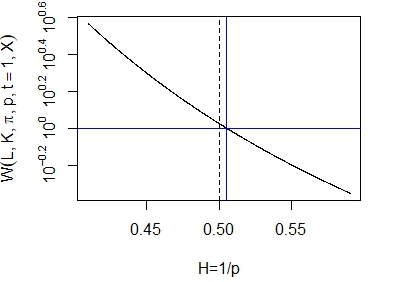
\includegraphics[width=\linewidth]{wagainstp_H05.png}
    \end{subfigure}
    \hfill
    \begin{subfigure}{0.48\textwidth}
        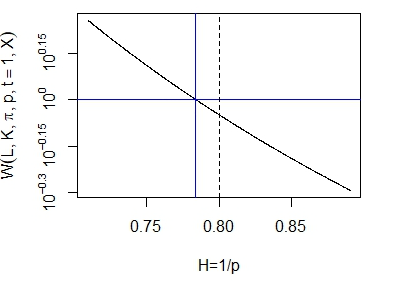
\includegraphics[width=\linewidth]{wagainstp_H08.png}
    \end{subfigure}
    
    \caption{Log-scale plot of the normalized $p$-th variation statistic for fBm with Hurst parameter $H=\{0.1,0.3,0.5,0.8\}$. The black solid line represents the value of $\log(W(L=300\times 300, K=300, \pi, p, t=1, X=B^H))$ plotted against $H=1/p$. The blue vertical line represents $\widehat{H}_{L,K}$ using the normalized $p$-th variation statistic with $L=300\times 300$ and $K=300$. The vertical black dotted line represents the true Hurst parameter. }
    \label{fig:checkw}
\end{figure}\\\\
We now repeat the estimation procedure for 150 independent sample paths using again $W(L=300\times 300, K=300, \pi, p, t=1, X=B^H)$. In Figure \ref{fig:checkhist} we have generated histograms of the final estimates $\widehat{H}_{L,K}$ for these 150 independent paths. In addition to this, we provide the corresponding summary statistics of the estimated roughness index $\widehat{H}_{L,K}$ for the 150 paths in Table \ref{tab:checkhist}. \\\\
Figure \ref{fig:checkw}, \ref{fig:checkhist} and Table \ref{tab:checkhist} all indicate that the estimated roughness index via $p$-th variation $\widehat{H}_{L,K}$ seems to be a fairly accurate roughness estimator when used on a data set with of $L=300\times 300$ generated from the fractional Brownian motion. All the roughness estimates $\widehat{H}_{L,K}$ are within a distance $0.05$ from the true Hurst parameter as seen in Figure \ref{fig:checkhist}. The mean and median of the estimated roughness provided in Table \ref{tab:checkhist} are in all four cases very close to the true Hurst parameter. However, for the fBm with Hurst parameter $H=0.8$ even the upper quartile of $\widehat{H}_{L,K}$ is smaller than the true Hurst parameter. This suggest that the estimated roughness index might be slightly biased downwards in the case of $H=0.8$. The estimate is, however, still quite accurate also for $H=0.8$, and we conclude that the roughness estimator $\widehat{H}_{L,K}$ performs very well in these simulation examples.
\begin{figure}[htbp]
    \centering
    
    \begin{subfigure}{0.48\textwidth}
        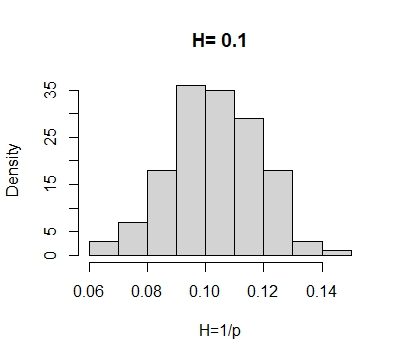
\includegraphics[width=\linewidth]{hist_H01.jpeg}
    \end{subfigure}
    \hfill
    \begin{subfigure}{0.48\textwidth}
        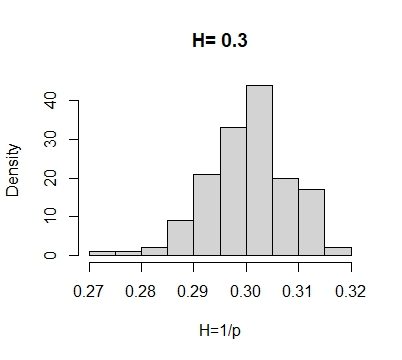
\includegraphics[width=\linewidth]{hist_H03.jpeg}
    \end{subfigure}
    \vskip -1em
    \begin{subfigure}{0.48\textwidth}
        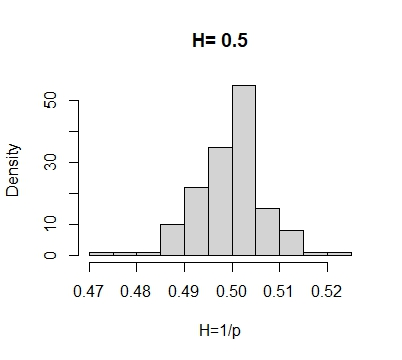
\includegraphics[width=\linewidth]{hist_H05.jpeg}
    \end{subfigure}
    \hfill
    \begin{subfigure}{0.48\textwidth}
        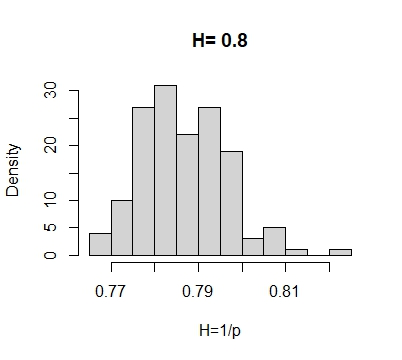
\includegraphics[width=\linewidth]{hist_H08.jpeg}
    \end{subfigure}
    
    \caption{Histogram of estimated roughness index $\widehat{H}_{L,K}$ with $L=300\times 300$ and $K=300$ generated from 150 independent simulation of fractional Brownian motions with Hurst parameter $H=\{0.1,0.3,0.5,0.8\}$. }
    \label{fig:checkhist}
\end{figure}\\
\begin{table}[htbp]
    \centering
    \begin{tabular}{ccccccc}
        \toprule
        H & Min. & Lower quartile & Median & Mean & Upper quartile & Max. \\
        \midrule
        0.1 & 0.0622 & 0.0944 & 0.1021 & 0.1031 & 0.1149 & 0.1402 \\
        0.3 & 0.2746 & 0.2954 & 0.3012 & 0.3005 & 0.3052 & 0.3177 \\
        0.5 & 0.4743 & 0.4954 & 0.5004 & 0.4997 & 0.5041 & 0.5239 \\
        0.8 & 0.7657 & 0.7797 & 0.7856 & 0.7865 & 0.7937 & 0.8239 \\
        \bottomrule
    \end{tabular}
    \caption{Summary of statistics for estimated roughness index $\widehat{H}_{L,K}$ from 150 independent simulations of fBm with $L=300\times 300$ and $K=300$.}
    \label{tab:checkhist}
\end{table}\\
We now set $L=2000\times 2000$ and $K=2000$, and simulate data from a fBm with Hurst parameter $H=0.1$. We compute $\hat{H}_{L,K}$ and as before we generate a histogram of the roughness estimates based on 150 independent paths. The results are presented in Figure \ref{fig:check2000}. Table \ref{tab:check2000} provides the summary statistics for the estimated roughness index $\widehat{H}_{L,K}$ corresponding to the histogram in Figure \ref{fig:check2000}. We observe that the results are similar to those we obtained for $L=300\times 300$ and $K=300$ but that the estimated roughness index $\hat{H}_{L,K}$ seems to be even more accurate. This is not surprising since we know that the normalized $p$-th variation statistic converges to the normalized $p$-th variation as $L$ and $K$ increase. However, increasing $L$ and $K$ is also computationally more demanding. The accuracy of $\widehat{H}_{L,K}$ obtained when using $L=300\times 300$ and $K=300$ is also satisfactory for many purposes in this thesis.
\begin{figure}[htbp]
    \centering
    
    \begin{subfigure}{0.48\textwidth}
        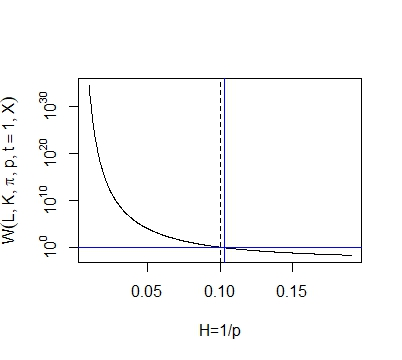
\includegraphics[width=\linewidth]{H01_2000_1.jpeg}
    \end{subfigure}
    \hfill
    \begin{subfigure}{0.48\textwidth}
        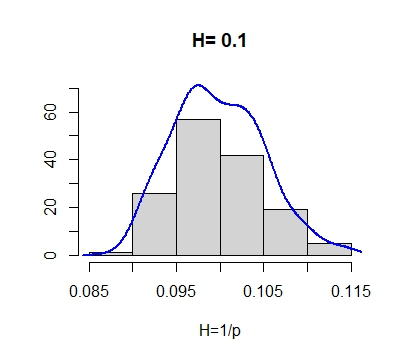
\includegraphics[width=\linewidth]{H01_2000_2.jpeg}
    \end{subfigure}
    
    \caption{Simulation results for fractional Brownian motion with Hurst parameter $H=0.1$. \textbf{Left:} The value of $\log(W(L=2000\times 2000, K=2000, \pi, p, t=1, X=B^H))$ plotted against $H=1/p$ in black. The blue vertical line represents the estimated roughness $\hat{H}_{L,K}$ using $L=2000\times 2000$ and $K=2000$. The vertical black dotted line represents the true Hurst parameter. \textbf{Right:} Histogram of estimated roughness index $\widehat{H}_{L,K}$ using $L=2000\times 2000$ and $K=2000$ generated by 150 independent simulations of fBm with Hurst parameter $H=0.1$. The blue line represents a kernel estimator for density. }
    \label{fig:check2000}
\end{figure}\\
\begin{table}[htbp]
    \centering
    \begin{tabular}{ccccccc}
        \toprule
        H & Min. & Lower quartile & Median & Mean & Upper quartile & Max. \\
        \midrule
        0.1 & 0.0892 & 0.0963 & 0.0996 & 0.0998 & 0.1031 & 0.1145 \\
        \bottomrule
    \end{tabular}
    \caption{Summary of statistics for estimated roughness index $\widehat{H}_{L,K}$ from 150 independent simulations of fBm with $H=0.1$, $L=2000\times 2000$ and $K=2000$.}
    \label{tab:check2000}
\end{table}\\
We further investigate how the choice of $K<<L$ affects the estimated roughness index $\hat{H}_{L,K}$. In Figure \ref{fig:checkk}, we have plotted the estimated roughness $\hat{H}_{300\times 300,K}$ for a fractional Brownian motion with Hurst parameter $H=0.1$ for different values of $K$ with a fixed $L=300\times 300$. Note that when $\frac{L}{K}$ is not an integer, the $K$ many groups from the definition of normalized $p$-th variation statistic \eqref{eq:w_stat_def} do not contain exactly $\frac{L}{K}$ consecutive points. The code is implemented such that each group will contain either $\lceil \frac{L}{K} \rceil$ or $\lfloor \frac{L}{K} \rfloor$ consecutive points. Figure \ref{fig:checkk} shows that when $K$ is too low, the estimator $\hat{H}_{300\times 300,K}$ seems to be underestimating the true Hurst parameter whereas when $K$ is too high the Hurst parameter is overestimated. For $K\approx \sqrt{L}$ the estimated roughness index is quite consistent and close to the true Hurst parameter $H=0.1$. It is thus natural to use $K=\sqrt{L}$ since $\frac{L}{K}$ will be an integer and the estimator $\widehat{H}_{L,K}$ seems to be accurate and consistent in that range.
\begin{figure}[htbp]
    \centering
    
    \begin{subfigure}{0.78\textwidth}
        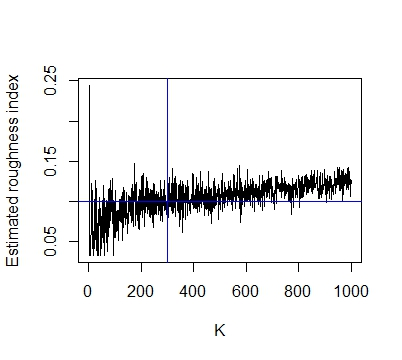
\includegraphics[width=\linewidth]{differentK.jpeg}
    \end{subfigure}
    
    \caption{The solid black line represents the estimated roughness index $\hat{H}_{300\times 300,K}$ plotted against different values of $K$ for a simulation from a fBm with Hurst parameter $H=0.1$. The blue vertical line represents $K=\sqrt{L}=300$ whereas the blue horizontal line represents the true Hurst parameter $H=0.1$.}
    \label{fig:checkk}
\end{figure}\\\\
In summary, these simulation examples show that for realistic sample sizes and frequencies encountered in high-frequency financial data, the roughness estimator via $p$-th variation $\widehat{H}_{L,K}$ is quite accurate and not sensitive to the block size $K$ in the range $K\approx \sqrt{L}$.

\subsection{Roughness estimator via logarithmic regression} 
In this section we will introduce the smoothness estimator via logarithmic regression used in \cite{gatheral}. Consider a volatility process on a time grid $[0,T]$. First we pretend that we have access to discrete observations of the spot volatility process with mesh $\Delta$ such that the observations are $\sigma_0, \sigma_\Delta, ..., \sigma_{k\Delta},...$ for $k \in \{0, \lfloor T / \Delta \rfloor\}$. Here $\Delta$ is a natural number and $\Delta\geq 1$. If we set $N=\lfloor T / \Delta \rfloor$, then for $q\geq 0$ we define
\begin{align*}
m(q,\Delta) = \frac{1}{N} \sum_{k=1}^N \lvert \log(\sigma_{k\Delta})-\log(\sigma_{(k-1)\Delta})\rvert^q.
\end{align*}
Following \cite{gatheral} the main assumption is that for some $s_q>0$ and $b_q>0$
\begin{align}
N^{qs_q}m(q,\Delta)\to b_q
\end{align}
as $\Delta$ tends to zero. Under additional technical assumptions, this essentially means that the volatility process belongs to a Besov smoothness space $\mathcal{B}^{s_q}_{q,\infty}$ and does not belong to $\mathcal{B}^{s_q'}_{q,\infty}$ for $s_q'>s_q$. Hence, $s_q$ can be considered as a smoothness parameter. In particular, if $\log(\sigma_t)$ is a fractional Brownian motion with Hurts parameter $H$, then for any $q\geq 0$  equation (17) holds in probability with $s_q=H$. It can further be shown that the sample paths of the process do indeed belong to $\mathcal{B}^{s_q}_{q,\infty}$. Thus, $s_q$ is a measure of the smoothness (or roughness) of the volatility process \cite{gatheral}.\\\\
The instantaneous volatility can not be directly observed, and exact computations of $m(q,\Delta)$ is not possible in practice.  In order to make use of $m(q,\Delta)$ we must therefore approximate the true spot volatility. The estimated volatility can be computed by the realized volatility or some variation of realized volatility. In the following we will be using the notation $m(q, \Delta)$ with the understanding that we are only approximating the true spot volatility. To estimate the smoothness parameter $s_q$ for each $q$, we can compute $m(q,\Delta)$ for different values of $\Delta$ and regress $\log m(q,\Delta)$ against $\log \Delta$. Note that for a given $\Delta$ several $m(q,\Delta)$ can be computed depending on the starting point. For example, if $\Delta=3$ then the starting point can be $\hat{\sigma}_0$, $\hat{\sigma}_{\Delta}$ or $\hat{\sigma}_{2\Delta}$. The final measure of $m(q,\Delta)$ is computed as the average of these values of $m(q,\Delta)$ with different starting points.\\\\
\cite{gatheral} shows that for a given $q$, $\log m(q,\Delta)$ values regressed against $\log \Delta$ essentially lie on a straight line. Assuming stationary increments of the log-volatility, this implies that the increments fulfil the scaling property 
\begin{align*}
\mathbb{E}\left[ \lvert \log (\sigma_\Delta) - \log (\sigma_0) \rvert^q\right] = b_q\Delta^{\zeta _q}
\end{align*}
where $\zeta_q = qs_q>0$ is the slope of the line associated to $q$. This result uses that $m(q,\Delta)$ can be seen as the empirical counterpart of $\mathbb{E}\left[ \lvert \log (\sigma_\Delta) - \log (\sigma_0) \rvert^q\right]$. Furthermore, \cite{gatheral} shows that $s_q$ seems to not depend on $q$, and plotting $\zeta_q$ against $q$ shows $\zeta_q \sim qs_q$.\\\\
Thus, we can compute an estimate of the smoothness (or roughness) of a volatility process by first regressing $\log m(q,\Delta)$ against $\log \Delta$ for different values of $q$. The slope of the straight line is an estimate of $\zeta_q$. Next, we regress $\zeta_q$ against $q$. The slope of the straight line is and estimate of the smoothness parameter $s_q$. If $\log(\sigma_t)$ is a fractional Brownian motion then $s_q=H$ holds in probability where $H$ is the Hurst parameter.\\\\
In Figure \ref{fig:oxfordlog} we have replicated the method used in \cite{gatheral} to estimate the roughness index of the volatility of S\&P500 using the first 3500 days of the daily realized variance estimates from the Oxford-Man Institute of Quantitative Finance Realized Library for S\&P. Our results coincide with the results from \cite{gatheral}, and the log-regression yields a straight line for all our values of $q$. Our estimated smoothness of the S\&P500 volatility is $H=0.1421$.
\begin{figure}[htbp]
    \centering
    
    \begin{subfigure}{0.48\textwidth}
        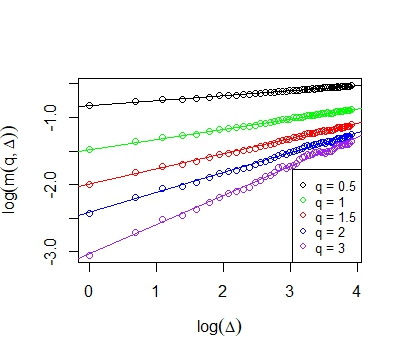
\includegraphics[width=\linewidth]{volis1.jpeg}
    \end{subfigure}
    \hfill
    \begin{subfigure}{0.48\textwidth}
        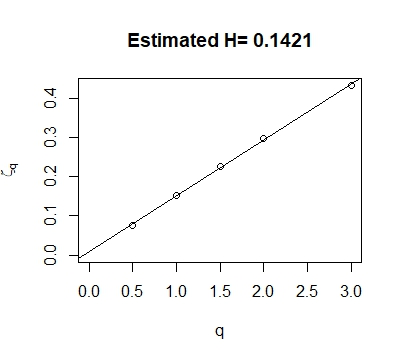
\includegraphics[width=\linewidth]{volis2.jpeg}
    \end{subfigure}
    
    \caption{A reproduction of the log-regression method introduced by \cite{gatheral} using the first 3500 days of the daily realized variance estimates from the Oxford-Man Institute of Quantitative Finance Realized Library for S\&P. The estimated roughness is $H=0.1421$. }
    \label{fig:oxfordlog}
\end{figure}\\
In Figure \ref{fig:oxfordw} we have used the roughness estimator from section 3.1 on the same S\&P500 volatility data to estimate the roughness. We have used $W(L = 3500, K = \sqrt{3500}, \pi, p, t=1, X)$ since the dataset only consist of 3500 days. We have set $t=1$ since $t$ simply works as a scaling parameter. The conclusions are the same for $t=1$ as for $t=3500$. The estimated roughness index is $\hat{H}_{L,K}=0.1425$. We immediately observe that the estimated roughness index is very close to the estimated smoothness parameter from the log-regression method $s_q=0.1421$. However, note that $L=3500$ is much smaller than $L=300\times 300 = 90000$ for which we have investigated the accuracy of the roughness estimator via normalized $p$-th variation statistic. Therefore, the estimated roughness estimator $\hat{H}_{L,K}$ might not be very precise. The results do however indicate that our two different approaches to estimate the roughness of a volatility process coincides.
\begin{figure}[htbp]
    \centering
    
    \begin{subfigure}{0.78\textwidth}
        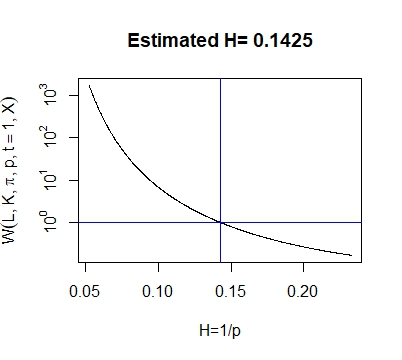
\includegraphics[width=\linewidth]{volisW.jpeg}
    \end{subfigure}
    
    \caption{Estimating the roughness of the first 3500 days of S\&P500 volatility data from Oxford-Man Institute of Quantitative Finance Realized Library using the roughness estimator from section 3.1 with $L=3500$ and $K=\sqrt{3500}$. The estimated roughness index is $\hat{H}_{L,K}=0.1425$.}
    \label{fig:oxfordw}
\end{figure}\\

\subsection{Sequential scale estimator of roughness exponent}
The third estimator we will introduce, is the sequential scale estimator of roughness first introduced by \cite{han}. This estimator differs from many other roughness estimators by the fact that it is computed directly from discrete observations of realized variance. That is, the input to the estimator needs to be realized variance and not instantaneous variance or volatility. The two previously described estimators are based on having access to discrete observations of instantaneous volatility $\sigma_t$. Realized volatility is then used as an approximation of the true spot volatility. This two step approach can be problematic since the estimation error in the realized volatility might substantially distort the outcome of the final roughness estimation. The sequential scale estimator avoids these possible inaccuracies caused by the estimation errors since it is based directly on realized variance.\\\\
\cite{han} are mainly concerned with stochastic volatility models based on fractional Brownian motions, but many aspects of the approach works in a model-free setting. Let $x: [0,1] \rightarrow \mathbb{R}$ be any continuous function. For $p\geq 1$ the $p$-th variation of the function $x$ along the $n$-th dyadic partition is defined as
\begin{align*}
\langle x \rangle^{(p)}_n := \sum_{k=0}^{2^n-1} \lvert x((k+1)2^{-n})-x(k2^{-n})\rvert^p.
\end{align*}
The above definition is similar to Definition 1. If there exist a $R\in [0,1]$ such that
\begin{align*}
\lim_{n\rightarrow\infty}\langle x \rangle^{(p)}_n =
\begin{cases} 
0 & \text{for } p > \frac{1}{R} \\
\infty & \text{for } p < \frac{1}{R}
\end{cases}
\end{align*}
we refer to $R$ as the roughness exponent of $x$. The smaller $R$ the rougher is the path $x$ and vice verse. Moreover, if $x$ is a sample path of a fractional Brownian motion, the roughness exponent R is equal to the Hurst parameter $H$ \cite{han}.\\\\
Now, since only asset prices and their realized variance can be observed in practice, we can consider this as making discrete observations of
\begin{align}
y(t) = \int_0^t g\left(x(s)\right) ds, \quad 0\leq t \leq 1, \label{eq:intvar}
\end{align}
where $g: \mathbb{R}\rightarrow \mathbb{R}$ is sufficiently regular. Here $y(t)$ shall be seen as integrated variance. Therefore, $g(x(t))$ should represent the variance of the underlying model. For instance, if log-volatility is given by a fractional Ornstein-Uhlenbeck process, we will take $x$  as a sample path of a fractional Ornstein-Uhlenbeck process and $g(t)=(e^t)^2 = e^{2t}$.\\\\
For the estimator, it is supposed that for a given $n\in \mathbb{N}$ we have access to the discrete observations $\{y(k2^{-n-2}):k=0,...,2^{n+2}\}$ of the integrated variance (i.e. the function $y$ in (\ref{eq:intvar})). Based on these data points, the following coefficients are introduced
\begin{align}
\vartheta_{n,k} := 2^{3n/2+3} \left( 
y\left( \frac{4k}{2^{n+2}} \right) 
- 2y\left( \frac{4k+1}{2^{n+2}} \right) 
+ 2y\left( \frac{4k+3}{2^{n+2}} \right) 
- y\left( \frac{4k+4}{2^{n+2}} \right) 
\right),
\end{align}
for $0\leq k \leq 2^n - 1$. The estimator for the roughness exponent is then given by
\begin{align*}
\hat{\mathscr{R}}_n (y) := 1 - \frac{1}{n}\log_2 \sqrt{\sum_{k=0}^{2^n-1}\vartheta_{n,k}^2}.
\end{align*}
Detailed explanation of the rationale behind the estimator can be seen in \cite{han} where convergence and consistency results are also shown.\\\\
The estimator $\hat{\mathscr{R}}_n (y)$ is not scale-invariant, and \cite{han} suggest to do scale-invariant modifications of $\hat{\mathscr{R}}_n (y)$. Fix $m\in \mathbb{N}$ with $n>m$ and fix $\alpha_0, ..., \alpha_m \geq 0$ with $\alpha_0>0$. The sequential scaling factor $\lambda_n^s$ is then defined as
\begin{align}
\lambda_n^s := \arg\min_{\lambda>0} \sum_{k=n-m}^n \alpha_{n-k} \left( \hat{\mathscr{R}}_k (\lambda y)-\hat{\mathscr{R}}_{k-1} (\lambda y)\right)^2 . \label{eq:scale_lambda}
\end{align}
The sequential scaling estimate $\hat{\mathscr{R}}_n^s (y)$ is then defined as follows 
\begin{align*}
\hat{\mathscr{R}}_n^s (y) := \hat{\mathscr{R}}_n (\lambda_n^s y).
\end{align*}
The idea is that the sequential scaling factor $\lambda_n^s$ enforces the convergence of $\hat{\mathscr{R}}_n (\lambda_n^s y)$. Thus, $\hat{\mathscr{R}}_n^s (y)$ will in some cases converge faster than $\hat{\mathscr{R}}_n (y)$ and remove bias. \cite{han} prove that the sequential scale estimator is scale-invariant and has a unique solution for every function $y\in C[0,1]$.\\\\
In practice the roughness exponent is usually estimated from realized variance rather than integrated variance. That is, realized variance is used as an approximation of integrated variance. Let $(m_n)_{n\in \mathbb{N}_0}$ be a fixed increasing sequence, where $m_n$ can be regarded as the number of observed data points used to compute the realized variance over each interval $[k2^{-n},(k+1)2^{-n}]$. Then we can denote the realized variance used for the sequential scale estimator in the following way
\begin{align}
\widehat{Y}_t^{(n)} := \sum_{k=1}^{\lfloor 2^nm_nt \rfloor} \left( \log S_{\frac{k}{2^n m_n}} - \log S_{\frac{k-1}{2^n m_n}}\right)^2 . \label{eq:rvforscale}
\end{align}
Thus, the process $\widehat{Y}_t^{(n)}$ is the realized variance calculated from the price process $S_t$ with a mesh size $(2^nm_n)^{-1}$. From $\widehat{Y}_t^{(n)}$ we can define the proxy coefficients $\widetilde{\vartheta}_{n,k}$ as
\begin{align*}
\widetilde{\vartheta}_{n,k} := 2^{3n/2+3} \left( 
\widehat{Y}_{ \frac{4k}{2^{n+2}}}^{(n+2)}
- 2\widehat{Y}_{\frac{4k+1}{2^{n+2}}}^{(n+2)}
+ 2\widehat{Y}_{\frac{4k+3}{2^{n+2}}}^{(n+2)} 
- \widehat{Y}_{\frac{4k+4}{2^{n+2}}}^{(n+2)} 
\right).
\end{align*}
By replacing $\vartheta_{n,k}$ with $\widetilde{\vartheta}_{n,k}$ we can construct an estimator $\widetilde{\mathscr{R}}_n (y)$ that directly estimates the roughness exponent from the realized variance as follows
\begin{align*}
\widetilde{\mathscr{R}}_n (S) := 1 - \frac{1}{n}\log_2 \sqrt{\sum_{k=0}^{2^n-1}\widetilde{\vartheta}_{n,k}^2}
\end{align*}
where $S$ denotes the price process that $\widetilde{\mathscr{R}}_n$ estimates from. \cite{han} show that under certain assumptions on the difference between $\widehat{Y}_t^{(n)}$ and $Y_t^{(n)}$, then $\widetilde{\mathscr{R}}_n (S)$ and $\hat{\mathscr{R}}_n (Y)$ converge to the same limit as $n$ increases provided that $m_n$ grows fast enough. We will by $\widetilde{\mathscr{R}}_n^s (S)$ denote the sequential scale estimator of realized variance which is defined as
\begin{align*}
\widetilde{\mathscr{R}}_n^s (\widehat{Y}_t^{(n)}) := \widetilde{\mathscr{R}}_n (\lambda_n^s \widehat{Y}_t^{(n)})
\end{align*} 
where $\lambda_n^s$ is computed in the same manner as (\ref{eq:scale_lambda}) just using $\widetilde{\mathscr{R}}_n(\widehat{Y}_t^{(n)})$ instead of $\widehat{\mathscr{R}}_n(Y)$.\\\\
We will now illustrate the performance of $\hat{\mathscr{R}}_n^s (y)$ and $\hat{\mathscr{R}}_n (y)$ in a simple example by replicating a simulation example from \cite{han}. We let $x$ follow a sample path of a fractional Brownian motion $B^H_t$ and set $g(x)=x$. For the computation of $\hat{\mathscr{R}}_n (y)$ we require observations of $y$ at all values of the time grid $\mathbb{T}_{n+2}:= \{k 2^{-n-2} : k=0,1,...,2^{n+2}\}$. In order to approximate $y(t)=\int_0^t B^H_s ds$ we are simulating the values of $B^H_t$ on a finer time grid $\mathbb{T}_N$ with $N=n+6$. Then we put
\begin{align}
Y_{k2^{-n-2}}:= 2^{-N} \sum_{j=1}^{2^{N-n-2}k} B^H_{j2^{-N}}, \quad k=0,1,...,2^{n+2} \label{eq:scaley}
\end{align}
which is an approximation of $y(t)=\int_0^t B^H_s ds$ by Riemann sums. In Figure \ref{fig:scaleplot} we display the results for the estimators $\hat{\mathscr{R}}_n $ and $\hat{\mathscr{R}}_n^s $ for 1000 independent paths of a fractional Brownian motion for different values of $n$. The left plot of Figure \ref{fig:scaleplot} is based on paths from a fractional Brownian motion with Hurst exponent $H=0.3$ while the right plot is for a fBm with $H=0.7$. The top plots are from the original estimator $\hat{\mathscr{R}}_n$ whereas the bottom plots are box plots of the sequential scale estimates $\hat{\mathscr{R}}_n^s (y)$. We observe from the top plots in Figure \ref{fig:scaleplot} that $\hat{\mathscr{R}}_n$ performs relatively well and seems to converge to the true roughness exponent as $n$ increases. However, the estimator also exhibits a certain bias. The corresponding results for the sequential scale estimator $\hat{\mathscr{R}}_n^s$ are displayed in the bottom plots of Figure \ref{fig:scaleplot}. We observe that by passing to the sequential scale estimator we completely remove the bias observed for $\hat{\mathscr{R}}_n$. Overall, $\hat{\mathscr{R}}_n^s $ seems to be a quite accurate estimate especially for $n\geq 15$. 
\begin{figure}[htbp]
    \centering
    
    \begin{subfigure}{0.48\textwidth}
        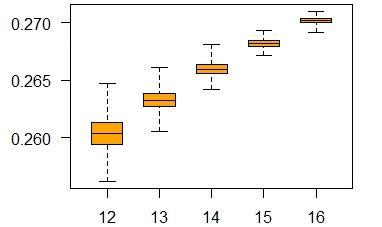
\includegraphics[width=\linewidth]{box3.png}
    \end{subfigure}
    \hfill
    \begin{subfigure}{0.48\textwidth}
        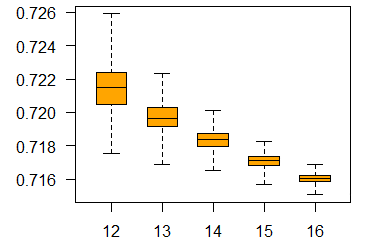
\includegraphics[width=\linewidth]{box1.png}
    \end{subfigure}
    \vskip 0em
    \begin{subfigure}{0.48\textwidth}
        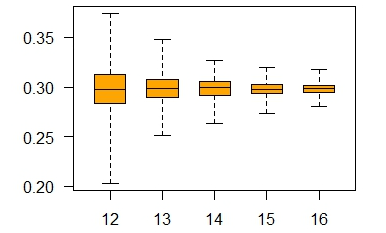
\includegraphics[width=\linewidth]{box4.png}
    \end{subfigure}
    \hfill
    \begin{subfigure}{0.48\textwidth}
        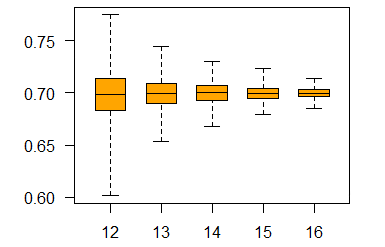
\includegraphics[width=\linewidth]{box2.png}
    \end{subfigure}
    
    \caption{Box plots of the original estimates $\hat{\mathscr{R}}_n (Y)$ (top) and the sequential scale estimates $\hat{\mathscr{R}}_n^s (Y)$ (bottom) for $n=12,...,16$ based on 1000 independent simulations of a fractional Brownian motion with $H=0.3$ (left) and $H=0.7$ (right) and with $Y$ as in (\ref{eq:scaley}). The other parameters are chosen to be $m=3$ and $\alpha_k = 1$ for $k=0,1,2,3$.} \label{fig:scaleplot}
\end{figure}\\
We now make a bit more complicated simulation example. We let log volatility, $\log\sigma_t$ be given by a fractional Ornstein-Uhlenbeck process on the form 
\begin{align}
dX_t = +\rho(\mu - X_t) \, dt + dB^H_t\label{eq:scale_fou}
\end{align}
where $B^H_t$ is a fractional Brownian motion. In this example we use the parameters $\rho=0.2$, $X_0=0$ and $\mu=2$. As input to the estimator we need discrete observations of 
\begin{align*}
\int_0^t \sigma^2_s ds = \int_0^t e^{2X_s} ds, \quad 0\leq t \leq 1.
\end{align*}
To this end, we take again $N=n+6$ and simulate the values of $X_t$ on the finer time grid $\mathbb{T}_{N}:= \{k 2^{-N} : k=0,1,...,2^{N}\}$ by an Euler scheme. We then compute
\begin{align}
Y_{k2^{-n-2}}:= 2^{-N} \sum_{j=1}^{2^{N-n-2}k} exp\left(2X_{j2^{-N}}\right), \quad k=0,1,...,2^{n+2} \label{eq:scaley_fou}
\end{align} 
as an approximation of $\int_0^t e^{2X_s} ds$. In Figure \ref{fig:scaleplot_fou} we display the results for the estimators $\hat{\mathscr{R}}_n$ and $\hat{\mathscr{R}}_n^s$ for 1000 independent paths of (\ref{eq:scale_fou}) with $n = 12,...,16$. The left plot of Figure \ref{fig:scaleplot_fou} is based on paths from a Ornstein-Uhlenbeck process with Hurst exponent $H=0.3$ while the right plot is for a fOU with $H=0.7$. The top plots are from the original estimator $\hat{\mathscr{R}}_n (y)$ whereas the bottom plots are box plots of the sequential scale estimates $\hat{\mathscr{R}}_n^s$. We observe from the top plots in Figure \ref{fig:scaleplot} that the original estimator $\hat{\mathscr{R}}_n$ performs poorly in this case. However, the sequential scale estimator $\hat{\mathscr{R}}_n^s$ performs almost as well as in the simple case illustrated in Figure \ref{fig:scaleplot}. This is likely due to tha fact that $g(t)=e^{2t}$ used in \eqref{eq:scaley_fou} substantially distort the scale of the underlying process. Since the original estimator is not scale-invariant this leads to poor estimates. However, passing to $\hat{\mathscr{R}}_n^s (y)$ seems to completely remedy this distortion. 
\begin{figure}[htbp]
    \centering
    
    \begin{subfigure}{0.48\textwidth}
        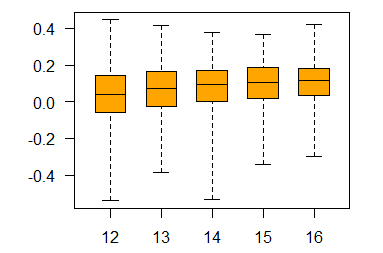
\includegraphics[width=\linewidth]{03fou_expo.png}
    \end{subfigure}
    \hfill
    \begin{subfigure}{0.48\textwidth}
        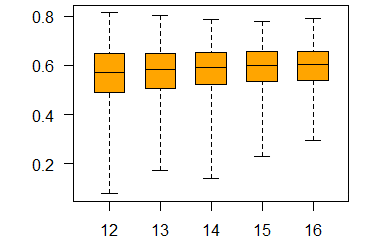
\includegraphics[width=\linewidth]{07fou_expo.png}
    \end{subfigure}
    \vskip 0em
    \begin{subfigure}{0.48\textwidth}
        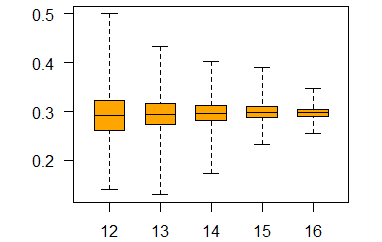
\includegraphics[width=\linewidth]{03fou_scale.png}
    \end{subfigure}
    \hfill
    \begin{subfigure}{0.48\textwidth}
        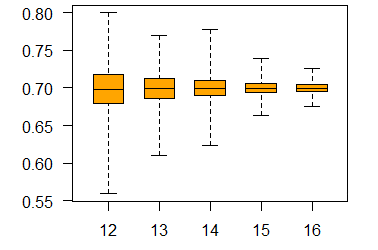
\includegraphics[width=\linewidth]{07fou_scale.png}
    \end{subfigure}
    
    \caption{Box plots of the original estimates $\hat{\mathscr{R}}_n (Y)$ (top) and the sequential scale estimates $\hat{\mathscr{R}}_n^s (Y)$ (bottom) for $n=12,...,16$ based on 1000 independent simulations of a fractional Ornstein-Uhlenbeck process \eqref{eq:scale_fou} with $H=0.3$ (left) and $H=0.7$ (right) and with $Y$ as in (\ref{eq:scaley_fou}). The other parameters are chosen to be $m=3$ and $\alpha_k = 1$ for $k=0,1,2,3$.} \label{fig:scaleplot_fou}
\end{figure}\\
Both of these simulation examples illustrate how the sequential scale estimator $\widehat{\mathscr{R}}_n^s$ improves the estimator $\widehat{\mathscr{R}}_n$. Overall, $\widehat{\mathscr{R}}_n^s$ seems to be performing very well and provide an accurate estimate of the true roughness of the underlying model especially for $n\geq 15$. We will be using $\widehat{\mathscr{R}}_n^s$ and $\widehat{\mathscr{R}}_n$ with $n\geq 15$ when performing numerical experiments in section 4.
\section{Numerical Experiments} \label{sec:num_exp}
In this section we will be performing a number of numerical experiments. We will be estimating the roughness index for stochastic models based directly on the instantaneous volatility $\sigma_t$ and based on the realized volatility by using price trajectories simulated from the models. By doing this we can investigate how estimation errors impact the estimated roughness index. We will be performing these experiments for stochastic models with various degrees of roughness.

\subsection{Simple stochastic volatility diffusion model}
First, we will consider the following stochastic volatility model where the volatility is the modulus of a Brownian motion:
\begin{align}
dS_t = \sigma_t S_t dB_t \quad \text{with} \quad \sigma_t = \lvert W_t \rvert, \label{eq:simple}
\end{align}
where $S_t$ is the price of the asset and $B_t$ and $W_t$ are two independent Brownian motions. For the simulation we use $S_0=1$ and $T=1$. The true roughness of this model is simply $H=0.5$.\\\\
We are estimating the realized variance using \eqref{eq:rvdef} for 300 consecutive points which corresponds to a 5 minute moving window when the price is updated every second. We estimate the roughness of the volatility process by using the realized volatility and instantaneous volatility as data in our roughness estimators. For every 300 consecutive points we are computing the realized volatility $RV_{t,t+\delta}(\pi^n)$ as in \eqref{eq:rvdef} and rescale the volatility to represents the same time interval as the corresponding instantaneous volatility $\sigma_t$. The corresponding instantaneous volatility is then the $\sigma_t$ for the first of these 300 points. In Figure \ref{fig:ex5IVRV}, we have made plots for the realized and instantaneous volatility. The left plot of Figure \ref{fig:ex5IVRV} represents the realized volatility of the price process in black and the instantaneous volatility in red. The middle plot of Figure \ref{fig:ex5IVRV} represents the difference between the realized and instantaneous volatility which is the estimation error. The right plot of Figure \ref{fig:ex5IVRV} represents the log difference between the realized and instantaneous volatility. Figure \ref{fig:ex5IVRV} indicates that the estimation error has a complicated dependence structure. There seems to be no obvious pattern in the estimation error and both the estimation error and log estimation error are far from I.I.D. 
\begin{figure}[h]
    \centering
    \begin{subfigure}{0.32\textwidth}
        \centering
        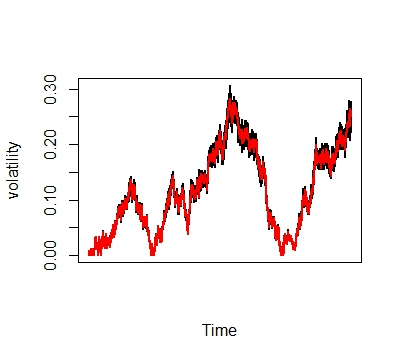
\includegraphics[width=\textwidth]{ex5_IVRV1.jpeg}
    \end{subfigure}\hfill
    \begin{subfigure}{0.32\textwidth}
        \centering
        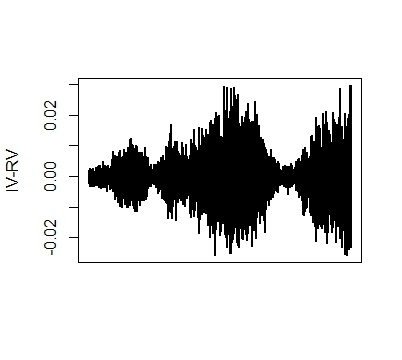
\includegraphics[width=\textwidth]{ex5_IVRV2.jpeg}
    \end{subfigure}\hfill
    \begin{subfigure}{0.32\textwidth}
        \centering
        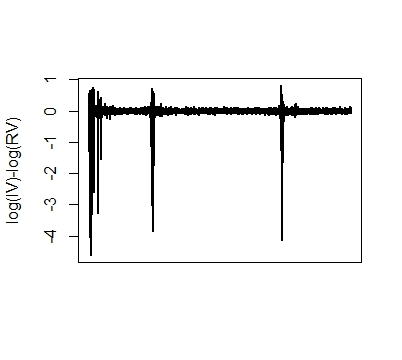
\includegraphics[width=\textwidth]{ex5_IVRV3.jpeg}
    \end{subfigure}
    \caption{Simulation from model \eqref{eq:simple}. \textbf{Left:} The red line represents instantaneous volatility $\sigma_t$ whereas the black line represents realized volatility $RV_t$. \textbf{Middle:} Corresponding estimation error for the left simulated path. \textbf{Right:} Corresponding log estimation error.}
    \label{fig:ex5IVRV}
\end{figure}\\\\
In Figure \ref{fig:ex5w} we have estimated the roughness index via normalized $p$-th variation from section 3.1 for realized and instantaneous volatility. In the left plot, we have used the realized volatility as data in the normalized $p$-th variation statistic and plotted $\log(W(K=500, L= 500\times 500, \pi, p, t=1, X = RV))$ against $H=\frac{1}{p}$. The right graph is a similar plot using instantaneous volatility instead of realized volatility. The obtained roughness estimators are very different for instantaneous and realized volatility. For realized volatility we obtain an estimated roughness of $\hat{H}_{L=500\times 500, K=500}(RV)=0.323$ which is much lower than the estimated roughness index for instantaneous volatility $\hat{H}_{L=500\times 500, K=500}(\sigma)=0.499$. The true roughness of the model is $H=0.5$. Thus, the roughness estimator is quite accurate when using instantaneous volatility which is in accordance with our results from section 3. However, the estimated roughness when using realized volatility is much rougher than the true roughness. As this is a simulation study we do have any measurement errors, and this rougher behaviour of realized volatility purely comes from the estimation error.
\begin{figure}[htbp]
    \centering
    
    \begin{subfigure}{0.48\textwidth}
        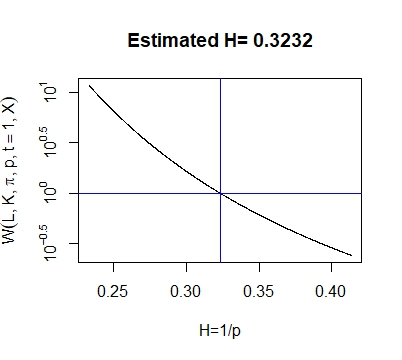
\includegraphics[width=\linewidth]{ex5_RVw.jpeg}
    \end{subfigure}
    \hfill
    \begin{subfigure}{0.48\textwidth}
        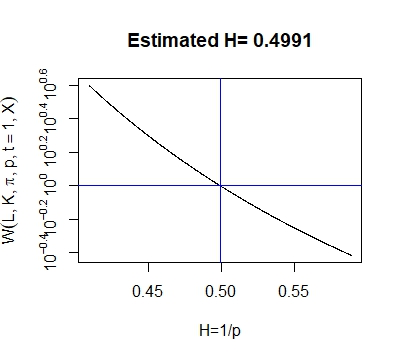
\includegraphics[width=\linewidth]{ex5_IVw.jpeg}
    \end{subfigure}
    
    \caption{The value of $\log(W(L=500\times 500, K=500, \pi, p, t=1, X))$ plotted against $H=1/p$ in black. The blue vertical line represents the estimated roughness $\hat{H}_{L,K}$. \textbf{Left:} Estimated roughness index $\hat{H}_{L,K}$ for realized volatility derived from the stochastic volatility model \eqref{eq:simple}. \textbf{Right:} Estimated roughness index for instantaneous volatility of the same price path.}
    \label{fig:ex5w}
\end{figure}\\\\
In Figure \ref{fig:ex5k} we have plotted the estimated roughness index $\hat{H}_{L=500\times 500,K}$ against different values of $K$. The left graph is for realized volatility while the right graph is for instantaneous volatility. The blue lines represents the estimated roughness $\hat{H}_{L,K}$ with $L=500\times 500$ and $K=500$ which are also reported in Figure \ref{fig:ex5w}. From the figure, we observe that irrespective of the choice of $K$ for the finite sample dataset of length $L=500\times 500$, the realized volatility is significantly rougher than the instantaneous volatility. The estimated roughness of the volatilities are quite consistent as long as $K$ is not too low for both volatilities. However, $\hat{H}_{L=500\times 500,K}$ seems to be even more consistent for instantaneous volatility than for the realized volatility.
\begin{figure}[htbp]
    \centering
    
    \begin{subfigure}{0.48\textwidth}
        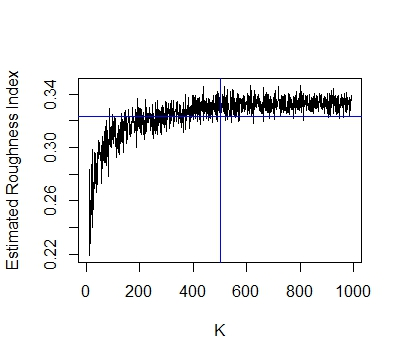
\includegraphics[width=\linewidth]{ex5_RVk.jpeg}
    \end{subfigure}
    \hfill
    \begin{subfigure}{0.48\textwidth}
        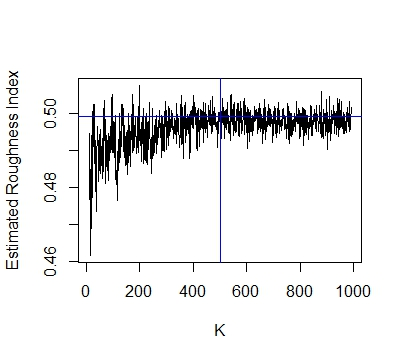
\includegraphics[width=\linewidth]{ex5_IVk.jpeg}
    \end{subfigure}
    
    \caption{The value of the estimated roughness index $\hat{H}_{L = 500\times 500 ,K}$ plotted against different values of $K$. \textbf{Left:} Estimated roughness index $\hat{H}_{L= 500\times 500,K}$ for realized volatility derived from the stochastic volatility model \eqref{eq:simple}. The horizontal blue line represents $\hat{H}_{L=500\times 500,K = 500} = 0.323$. \textbf{Right:} Estimated roughness index for instantaneous volatility of the same price path. The horizontal blue line represents $\hat{H}_{L=500\times 500,K = 500} = 0.499$.}
    \label{fig:ex5k}
\end{figure}\\\\
We now want to use the sequential scale estimator $\hat{\mathscr{R}}_n^s (y)$ to estimate the roughness for the same path that Figure \ref{fig:ex5w} was based on. The sequential scale estimator requires observations of integrated or realized variance $y(t) = \int_0^t g\left(x(s)\right) ds$ at all values of the time grid $\mathbb{T}_{n+2}:= \{k 2^{-n-2} : k=0,1,...,2^{n+2}\}$. To accommodate for that we rescale our simulated path from before. We will use $n=17$ for the roughness estimation. Now, to approximate $y$ properly we set $m_{17} = 2^5 = 32$ which is the number of data points in each interval $[k2^{-n},(k+1)2^{-n}]$. We then follow the procedure described in section 3.5 and make sure that we have values of the price process on the finer time grid $\mathbb{T}_{N}$ with $N=n+7$. Therefore, we need $2^N+1$ points on the time interval $t\in[0,1]$. Thus, for these points we have $\Delta t = 2^{-N}$. We rescale the first $2^N$ points of our simulated Brownian motions $B_t$ and $W_t$ such that they correspond to this new $\Delta t$. We then generate the price process as in (\ref{eq:simple}) using these rescaled Brownian motions. In Figure \ref{fig:ex5price} we have plotted the first 100000 data points of the original price process $S_t$ on the left and the corresponding rescaled price process on the right. We observe that the prices processes follow the exact same pattern. The only difference between the graphs is the axes that have been rescaled since we have rescaled the whole prices process. Therefore, we would expect the same roughness index of the two price processes. 
\begin{figure}[htbp]
    \centering
    
    \begin{subfigure}{0.48\textwidth}
        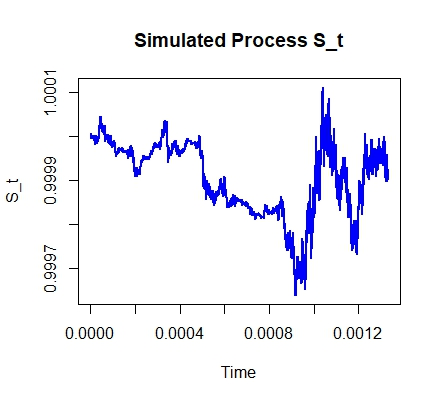
\includegraphics[width=\linewidth]{price_plot.jpeg}
    \end{subfigure}
    \hfill
    \begin{subfigure}{0.48\textwidth}
        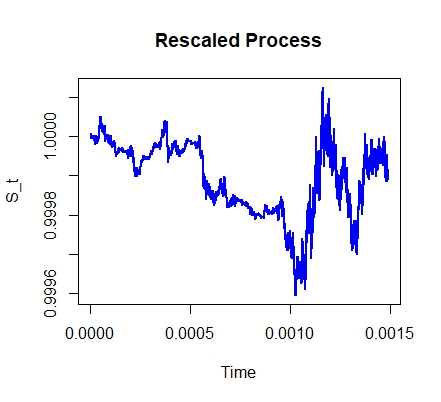
\includegraphics[width=\linewidth]{price_rescaled.jpeg}
    \end{subfigure}
    
    \caption{The first 100000 data points of the simulated price process $S_t$ generated from model (\ref{eq:simple}). The left plot is the original simulated path while the right plot is the rescaled price process with fewer points and a different mesh size used for the sequential scale estimator.}
    \label{fig:ex5price}
\end{figure}\\\\
We then compute the realized variance as in (\ref{eq:rvforscale}). In order to compare the realized variance/volatility with instantaneous volatility, we also approximate $y(t) = \int_0^t g\left(x(s)\right) ds$ directly from $\sigma_t$ by 
\begin{align}
Y_{k2^{-n-2}}:= 2^{-N} \sum_{j=1}^{2^{N-n-2}k} \sigma^2_{j2^{-N}}, \quad k=0,1,...,2^{n+2}. \label{eq:ex5y}
\end{align}
In Figure \ref{fig:ex5scale} we have plotted these two approximations of integrated variance $y(t)$ and their difference. The left plot of Figure \ref{fig:ex5scale} represent the realized variance in black and the approximation $Y$ directly from $\sigma_t$ as in (\ref{eq:ex5y}) in red. The middle plot shows the difference between these two approximations of integrated variance, and the right plot shows the difference between the log of the two approximations. Figure \ref{fig:ex5scale} indicates that these two ways of computing the integrated variance yield very similar results, and the difference between realized variance and $Y$ is very small. On the left plot it is difficult to distinguish the red and the black line from each other since they fall directly on top of each other. However, there is a small difference as seen on the two plots to the right, and especially the log difference is somewhat big in the very beginning when the integrated variance is very small.
\begin{figure}[h]
    \centering
    \begin{subfigure}{0.32\textwidth}
        \centering
        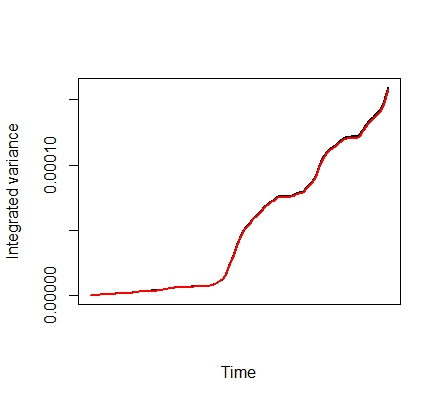
\includegraphics[width=\textwidth]{ex5_scale1.jpeg}
    \end{subfigure}\hfill
    \begin{subfigure}{0.32\textwidth}
        \centering
        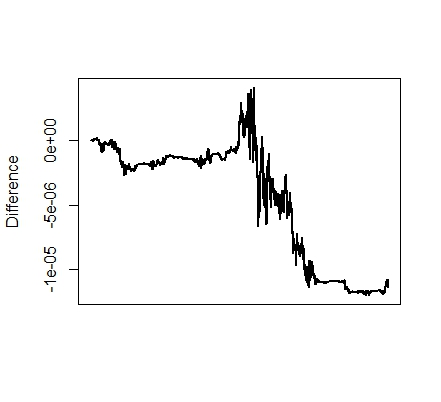
\includegraphics[width=\textwidth]{ex5_scale2.jpeg}
    \end{subfigure}\hfill
    \begin{subfigure}{0.32\textwidth}
        \centering
        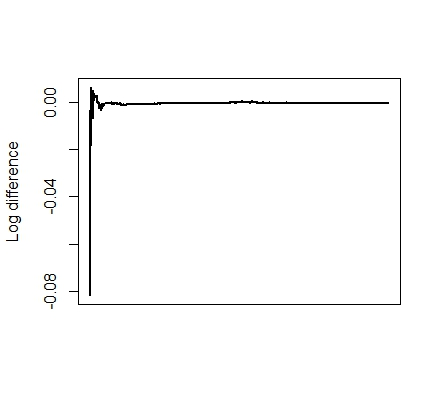
\includegraphics[width=\textwidth]{ex5_scale3.jpeg}
    \end{subfigure}
    \caption{Integrated variance of the original path from model \eqref{eq:simple} rescaled to fit the sequential scale estimator. \textbf{Left:} The red line represents $Y$ computed directly from instantaneous volatility $\sigma_t$ whereas the black line represents realized variance $\hat{Y}_t^{(n)}$. \textbf{Middle:} Corresponding difference between the lines in the left plot. \textbf{Right:} Corresponding log difference.}
    \label{fig:ex5scale}
\end{figure}\\\\
We now proceed to estimating the roughness by using respectively realized variance and spot variance $Y(\sigma_t)$. We denote the sequential scale estimator based directly on realized variance by $\widetilde{\mathscr{R}}_n^s (S)$ whereas the roughness estimated from $Y(\sigma_t)$ is denoted by $\widehat{\mathscr{R}}_n^s (Y)$. Table \ref{tab:ex5scaleest} provides the roughness estimates obtained from the sequential scale estimator for the rescaled path from model (\ref{eq:simple}). Furthermore, the table also provides the results from the original estimators $\widetilde{\mathscr{R}}_n (S)$ and $\widehat{\mathscr{R}}_n (Y)$ that are used for the computations of $\widetilde{\mathscr{R}}_n^s (S)$ and $\widehat{\mathscr{R}}_n^s (Y)$. Even though the difference between realized variance $\widehat{Y}_t^{(n)}$ and $Y(\sigma_t)$ is small, the sequential scale estimator yields very different results when used for these two variances as seen in Table \ref{tab:ex5scaleest}. The estimated roughness when using spot variance $Y(\sigma_t)$ is very close to the true roughness of the model $H=\frac{1}{2}$. However, when using realized variance the estimated roughness is $\widetilde{\mathscr{R}}_n^s (S)=-0.1073$ which is a value that roughness can never take. This indicates that the estimator $\widetilde{\mathscr{R}}_n^s (S)$ is very vulnerable to estimation errors in sense of difference between realized variance and integrated variance. This is surprising since the sequential scale estimator has been developed with the focus of avoiding the problems in roughness estimation caused by estimation errors. It is clear that the estimation error is smaller for the sequential scale estimator in the sense that the difference between realized variance $\widehat{Y}_t^{(n)}$ and $Y(\sigma_t)$ observed in Figure \ref{fig:ex5scale} is much smaller than the difference between realized volatility and instantaneous volatility observed in Figure \ref{fig:ex5IVRV}. However, the small difference between $\widehat{Y}_t^{(n)}$ and $Y(\sigma_t)$ is enough to substantially distort the outcomes of the roughness estimation. Furthermore, we observe from Table \ref{tab:ex5scaleest} that the original estimator $\widetilde{\mathscr{R}}_n(S)$ actually performs better than the sequential scale estimator $\widetilde{\mathscr{R}}_n^s(S)$ when used for realized variance. This is surprising since we illustrated in our simulation examples from section 3.5 how passing to the sequential scale estimator could remove bias and make the estimator converge faster. However, both $\widetilde{\mathscr{R}}_n^s(S)$ and $\widetilde{\mathscr{R}}_n(S)$ performs very poorly in this example.
\begin{table}[htbp]
    \centering
    \begin{tabular}{ccc}
        \toprule
         & Realized variance & Spot variance $Y(\sigma_t)$ \\
        \midrule
        Sequential scale estimator & $\widetilde{\mathscr{R}}_n^s (S) = -0.4938 $ & $\widehat{\mathscr{R}}_n^s (Y) = 0.5029$ \\
        Original scale estimator &$\widetilde{\mathscr{R}}_n (S) = 0.1813 $ & $\widehat{\mathscr{R}}_n (Y) = 0.5332$ \\
        Absolute scale estimator &$\lvert \widetilde{\mathscr{R}}_n^s (S)\rvert = 0.4938 $ & $\lvert \widehat{\mathscr{R}}_n^s (Y)\rvert = 0.5029$ \\
        \bottomrule
    \end{tabular}
    \caption{The roughness estimates from the sequential scale roughness estimator with $n=17$ and $m_{17}=2^5$ for model (\ref{eq:simple}) by using respectively realized variance and the approximation of integrated variance from instantaneous volatility $Y(\sigma_t)$. The results for the scale-invariant sequential scale estimator are displayed in the top row whereas the corresponding estimates from the original estimator are displayed in the bottom row.}
    \label{tab:ex5scaleest}
\end{table}\\\\
In Figure \ref{fig:ex5dens} we have repeated the estimation procedure across 150 independent paths drawn from model \eqref{eq:simple} and computed $\widehat{H}_{L,K}$, $\widetilde{\mathscr{R}}_n^s$, $\widehat{\mathscr{R}}_n$ and $\lvert \widetilde{\mathscr{R}}_n^s (S)\rvert$ for all paths. The left plot of Figure \ref{fig:ex5dens} displays density plots of the estimators when used on realized volatility and realized variance whereas the right plot displays density plots when using instantaneous volatility and $Y(\sigma_t)$ as input to the estimators. For $\widehat{H}_{L,K}$ we observe that when using realized volatility the estimator $\widehat{H}_{L,K}(RV)$ systematically underestimates the true roughness exponent of $H=\frac{1}{2}$. However, when used on instantaneous volatility $\widehat{H}_{L,K}(IV)$ is very accurate and estimates the true roughness of the model very well. 
\begin{figure}[htbp]
    \centering
    
    \begin{subfigure}{0.48\textwidth}
        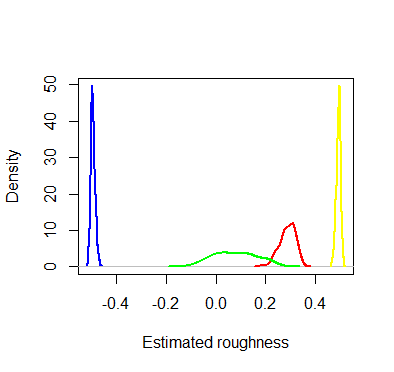
\includegraphics[width=\linewidth]{ex5_densRV.png}
    \end{subfigure}
    \hfill
    \begin{subfigure}{0.48\textwidth}
        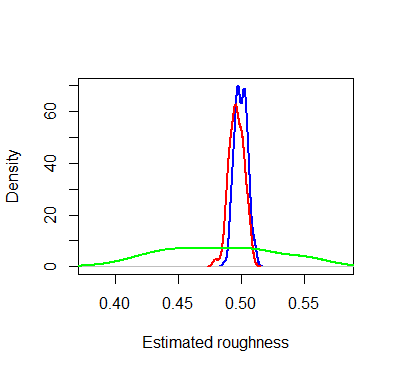
\includegraphics[width=\linewidth]{ex5_densIV.png}
    \end{subfigure}
    
    \caption{Density plots of the roughness estimators $\widehat{H}_{L,K}$ (red), $\widetilde{\mathscr{R}}_n^s$ (blue), $\widehat{\mathscr{R}}_n$ (green) and $\lvert \widetilde{\mathscr{R}}_n^s (S)\rvert$ (yellow) across 150 independent paths drawn from model \eqref{eq:simple}. \textbf{Left:} Using realized volatility and realized variance as input. \textbf{Right:} Using instantaneous volatility $\sigma_t$ and $Y(\sigma_t)$ as input.}
    \label{fig:ex5dens}
\end{figure}\\\\
\subsection{OU-SV model}
Now, we will simulate from the following OU-SV model:
\begin{align}
dS_t = S_t \sigma_t dB_t, \quad \sigma_t = \sigma_0 e^{Y_t}, \quad dY_t = -\gamma Y_t \, dt + \theta \, dB'_t, \label{eq:ousv}
\end{align}
where $S_t$ is the price of the asset and $B_t$ and $B_t'$ are two independent Brownian motions. In the simulation, we are using the parameters $\sigma_0=\gamma=\theta=1$ and $Y_0=0$ and we set $T=5$ and $S_0=1$. The true roughness of this model is $H=0.5$.\\\\
We are using the same procedure as described in section 4.1 to generate our realized and instantaneous volatility. In Figure \ref{fig:example}, we have made plots for these volatilities. The left plot of Figure \ref{fig:example} represents the realized volatility of the price process in black and the instantaneous volatility in red. The middle plot of Figure \ref{fig:example} represents the difference between the realized and instantaneous volatility which is the estimation error. The right plot of Figure \ref{fig:example} represents the log difference between the realized and instantaneous volatility. Visually the middle plot suggests that the estimation error has a complicated dependence structure. However, the log estimation error on the right plot of Figure \ref{fig:example} seems to have an I.I.D. Gaussian structure. This is supported by the theory in \cite{fukasawa}. However, as shown in Section 4.1 the I.I.D. behaviour of the log estimation error does not in general hold for stochastic diffusive models as assumed in \cite{fukasawa}. 
\begin{figure}[h]
    \centering
    \begin{subfigure}{0.32\textwidth}
        \centering
        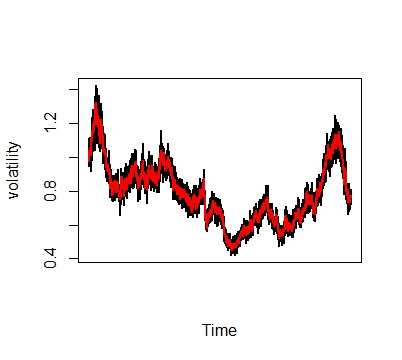
\includegraphics[width=\textwidth]{ex6_IVRV1.jpeg}
    \end{subfigure}\hfill
    \begin{subfigure}{0.32\textwidth}
        \centering
        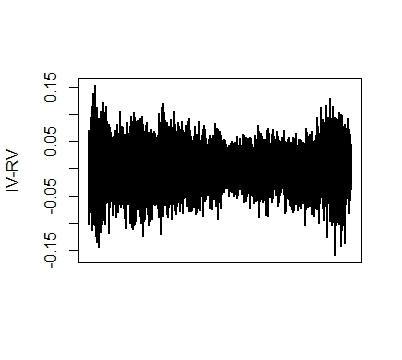
\includegraphics[width=\textwidth]{ex6_IVRV2.jpeg}
    \end{subfigure}\hfill
    \begin{subfigure}{0.32\textwidth}
        \centering
        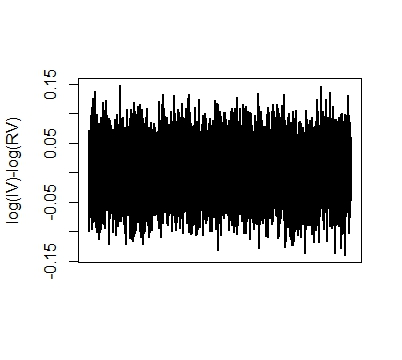
\includegraphics[width=\textwidth]{ex6_IVRV3.jpeg}
    \end{subfigure}
    \caption{Simulation from the OU-SV model. \textbf{Left:} The red line represents instantaneous volatility $\sigma_t$ whereas the black line represents realized volatility $RV_t$. \textbf{Middle:} Corresponding estimation error for the left simulated path. \textbf{Right:} Corresponding log estimation error.}
    \label{fig:example}
\end{figure}\\\\
In Figure \ref{fig:ex6w} we have estimated the roughness index via normalized $p$-th variation for realized and instantaneous volatility. In the left plot, we have used the realized volatility as input to the normalized $p$-th variation statistic and plotted $\log(W(K=300, L= 300\times 300, \pi, p, t=1, X = RV))$ against $H=\frac{1}{p}$. The right graph is a similar plot using instantaneous volatility instead of realized volatility. The obtained roughness estimators are very different for instantaneous and realized volatility. For realized volatility we obtain an estimated roughness of $\hat{H}_{L=300\times 300, K=300}(RV)=0.155$ which is much lower than the estimated roughness index for instantaneous volatility $\hat{H}_{L=300\times 300, K=300}(\sigma)=0.501$. The true roughness of the model is $H=0.5$. Thus, also for this example the roughness estimator is very accurate when using instantaneous volatility. However, the estimated roughness when using realized volatility is much rougher than the true roughness, and realized variance appear even rougher in this example compared to the previous one. As this is a simulation study this rougher behaviour of realized volatility purely comes from the estimation error, and this illustrates how estimation errors can substantially distort the roughness estimate.
\begin{figure}[htbp]
    \centering
    
    \begin{subfigure}{0.48\textwidth}
        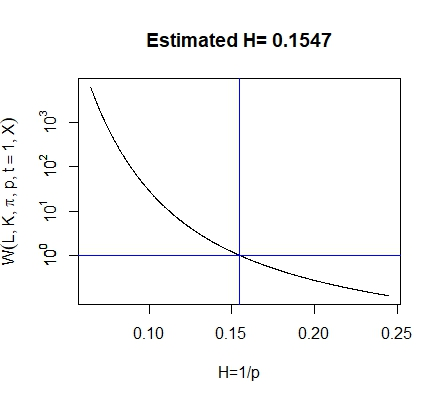
\includegraphics[width=\linewidth]{ex6_RVw.jpeg}
    \end{subfigure}
    \hfill
    \begin{subfigure}{0.48\textwidth}
        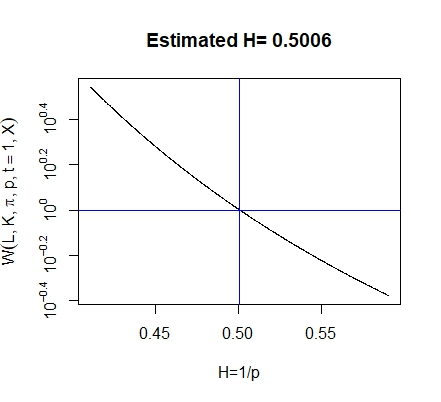
\includegraphics[width=\linewidth]{ex6_IVw.jpeg}
    \end{subfigure}
    
    \caption{The value of $\log(W(L=300\times 300, K=300, \pi, p, t=1, X))$ plotted against $H=1/p$ in black. The blue vertical line represents the estimated roughness $\hat{H}_{L,K}$. \textbf{Left:} Estimated roughness index $\hat{H}_{L,K}$ for realized volatility derived from the stochastic volatility model \eqref{eq:simple}. \textbf{Right:} Estimated roughness index for instantaneous volatility of the same price path.}
    \label{fig:ex6w}
\end{figure}\\\\
Now we use the roughness estimator by logarithmic regression $\hat{H}_R$ for the same instantaneous volatility and realized volatility data. In Figure \ref{fig:ex6logIV} we display the results for the roughness estimator when using instantaneous volatility. The estimated roughness index is $\hat{H}_R=0.498$ which is very close to the true roughness of the model $H=\frac{1}{2}$. This indicates that the roughness estimator performs well for instantaneous volatility. In Figure \ref{fig:ex6logRV} we display the corresponding results for the log regression estimator $\hat{H}_R$ when using realized volatility as input. Here we obtain an estimated roughness of $\hat{H}_R=0.089$ which is even rougher than the estimate we obtained for the estimator $\hat{H}_{L,K}$ via $p$-th variation. This rougher behaviour purely comes from the estimation error, and this once again illustrates that using realized volatility for roughness estimation can lead to a dramatic underestimation of the true roughness of the underlying model.
\begin{figure}[htbp]
    \centering
    
    \begin{subfigure}{0.48\textwidth}
        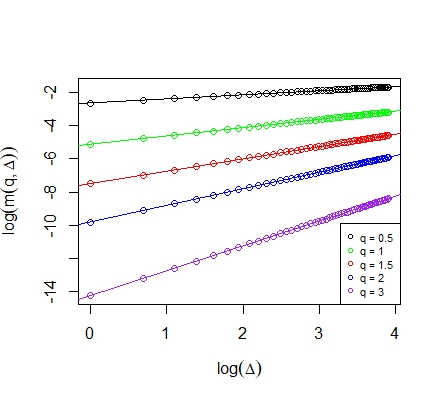
\includegraphics[width=\linewidth]{ex6_logIV1.jpeg}
    \end{subfigure}
    \hfill
    \begin{subfigure}{0.48\textwidth}
        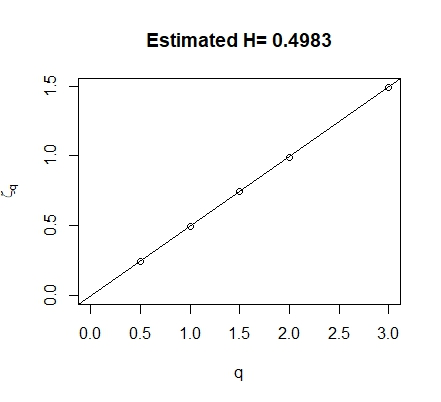
\includegraphics[width=\linewidth]{ex6_logIV2.jpeg}
    \end{subfigure}
    
    \caption{Roughness estimation by log regression using instantaneous volatility simulated from model \eqref{eq:ousv}. \textbf{Left:} $\log(m(q,\Delta))$ plotted against $\log(\Delta)$. \textbf{Right:} Regression coefficients $\zeta_q$ plotted against $q$. The estimated roughness index is $\hat{H}_R=0.498$.}
    \label{fig:ex6logIV}
\end{figure}\\\\
\begin{figure}[htbp]
    \centering
    
    \begin{subfigure}{0.48\textwidth}
        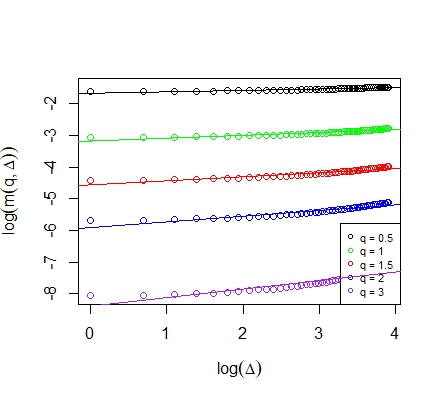
\includegraphics[width=\linewidth]{ex6_logRV1.jpeg}
    \end{subfigure}
    \hfill
    \begin{subfigure}{0.48\textwidth}
        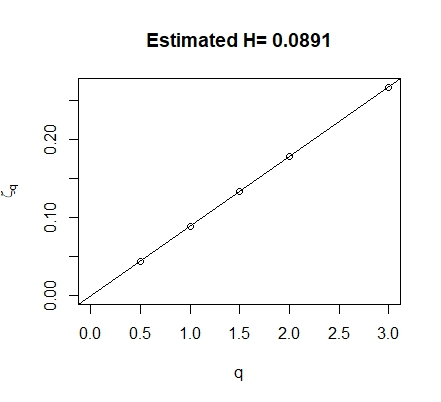
\includegraphics[width=\linewidth]{ex6_logRV2.jpeg}
    \end{subfigure}
    
    \caption{Roughness estimation by log regression using realized volatility for a price path simulated from model \eqref{eq:ousv}. \textbf{Left:} $\log(m(q,\Delta))$ plotted against $\log(\Delta)$. \textbf{Right:} Regression coefficients $\zeta_q$ plotted against $q$. The estimated roughness index is $\hat{H}_R=0.089$.}
    \label{fig:ex6logRV}
\end{figure}\\\\
We will now use the sequential scale estimator for the same price path. We will be using $n=17$ and $m_{17}=2^5$ for the estimation. Furthermore, we use the parameters $m=4$ and $\alpha_k=1$ for $k=0,1,2,3$ for the computation of $\widehat{\mathscr{R}}_n^s$. As in section 4.1 we will rescale the price process such that our observed data points fit the required input for the sequential scale estimator. To this end, we need $2^{n+7}$ data points on the time interval $[0,1]$. We set $dt=2^{-n-7}$ and rescale our $dB_t$ and $dB_t'$ to this new $dt$. We then compute $S_t$ as in \eqref{eq:ousv} using these rescaled $dt$, $dB_t$ and $dB_t'$. We compute realized variance $\hat{Y}_t^{(n)}$ as in \eqref{eq:rvforscale} and $Y(\sigma_t)$ as in \eqref{eq:ex5y}. \\
In Figure \ref{fig:ex6scale} we have plotted these two approximations of integrated variance $y(t)$ and their difference. The left plot of Figure \ref{fig:ex5scale} represent the realized variance in black and the approximation $Y(\sigma_t)$ as in (\ref{eq:ex5y}) in red. The middle plot shows the difference between these two approximations of integrated variance, and the right plot shows the difference between the log of the two approximations. Just as in the previous example we observe that these two ways of computing the integrated variance yield very similar results, and the difference between realized variance $\hat{Y}_t^{(n)}$ and $Y(\sigma_t)$ is very small. However, the log difference is much bigger in the very beginning when the integrated variance is very small.
\begin{figure}[h]
    \centering
    \begin{subfigure}{0.32\textwidth}
        \centering
        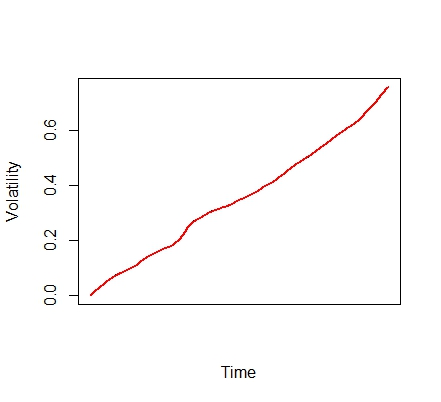
\includegraphics[width=\textwidth]{ex6_scale1.jpeg}
    \end{subfigure}\hfill
    \begin{subfigure}{0.32\textwidth}
        \centering
        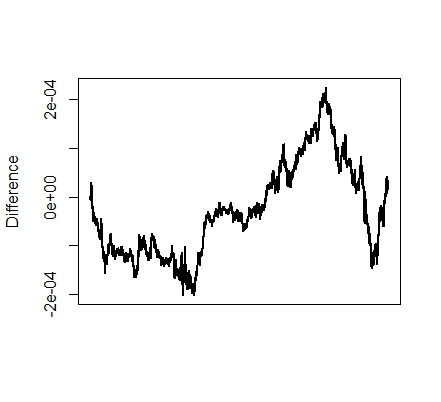
\includegraphics[width=\textwidth]{ex6_scale2.jpeg}
    \end{subfigure}\hfill
    \begin{subfigure}{0.32\textwidth}
        \centering
        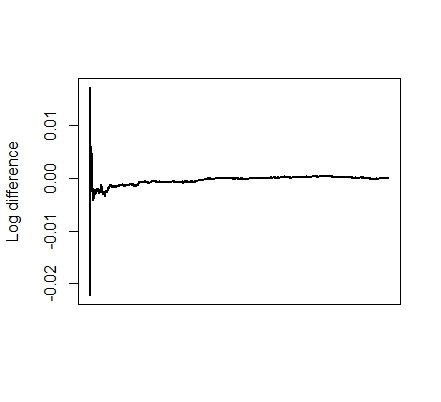
\includegraphics[width=\textwidth]{ex6_scale3.jpeg}
    \end{subfigure}
    \caption{Integrated variance of the original path from model \eqref{eq:ousv} rescaled to fit the sequential scale estimator. \textbf{Left:} The red line represents $Y$ computed directly from instantaneous volatility $\sigma_t$ whereas the black line represents realized variance $\hat{Y}_t^{(n)}$. \textbf{Middle:} Corresponding difference between the lines in the left plot. \textbf{Right:} Corresponding log difference.}
    \label{fig:ex6scale}
\end{figure}\\\\
In Table \ref{tab:ex6scaleest} we display the result from the sequential scale roughness estimation. As in the previous example we observe that the sequential scale estimator $\widehat{\mathscr{R}}_n^s$ provides an accurate roughness estimation close to the true roughness of the model $H=\frac{1}{2}$ when using $Y(\sigma_t)$ as input. It also significantly improves the original scale estimator $\widehat{\mathscr{R}}_n$. However, when using realized variance as input we obtain the roughness estimate $\widetilde{\mathscr{R}}_n^s (S) = -0.5012$ for the sequential scale estimator which is close to the negative of the true roughness of the model. The small difference between $\hat{Y}_t^{(n)}$ and $Y(\sigma_t)$ observed in Figure \ref{fig:ex6scale} completely changes the estimates $\widehat{\mathscr{R}}_n^s$ and $\widehat{\mathscr{R}}_n$. However, when simply using $\lvert \widetilde{\mathscr{R}}_n^s \rvert$ we obtain a very accurate roughness estimate for both realized variance and $Y(\sigma_t)$. These results indicate that $\lvert \widetilde{\mathscr{R}}_n^s \rvert$ could be a very robust estimator that is unaffected by the estimation error between realized and integrated variance.
\begin{table}[htbp]
    \centering
    \begin{tabular}{ccc}
        \toprule
         & Realized variance & Spot variance $Y(\sigma_t)$ \\
        \midrule
        Sequential scale estimator & $\widetilde{\mathscr{R}}_n^s (S) = -0.5012 $ & $\widehat{\mathscr{R}}_n^s (Y) = 0.4988$ \\
        Original scale estimator &$\widetilde{\mathscr{R}}_n (S) = 0.0529 $ & $\widehat{\mathscr{R}}_n (Y) = 0.5407$ \\
        Absolute scale estimator &$\lvert \widetilde{\mathscr{R}}_n^s (S)\rvert = 0.5012 $ & $\lvert \widehat{\mathscr{R}}_n^s (Y)\rvert = 0.4988$ \\
        \bottomrule
    \end{tabular}
    \caption{The roughness estimates from the sequential scale roughness estimator with $n=17$ and $m_{17}=2^5$ for model (\ref{eq:ousv}) by using respectively realized variance and the approximation of integrated variance from instantaneous volatility $Y(\sigma_t)$.}
    \label{tab:ex6scaleest}
\end{table}\\\\
We now compute the distributions of the estimated roughness index via normalized $p$-th statistic $\hat{H}_{L,K}$ with $L=300\times 300$ and $K=300$ for realized volatility and instantaneous volatility. We generate the distributions across 2500 independent paths drawn from the OU-SV model \eqref{eq:ousv}. The left plot of Figure \ref{fig:ex6dens} is the distribution of $\hat{H}_{L,K}$ for realized volatility whereas the right plot is the corresponding distribution for instantaneous volatility as data in the roughness estimator. In addition to this, Table \ref{tab:ex6dens} provides the summary statistics for the roughness estimator $\hat{H}_{L,K}$ for realized and instantaneous volatility respectively across the 2500 independent paths. We observe that realized volatility systematically exhibit much rougher behaviour than instantaneous volatility. The roughness estimates based on instantaneous volatility are very close to the roughness of the true model $H=0.5$. However, the roughness estimates generated from realized volatility are much smaller with a mean of $\hat{H}_{L,K}=0.1549$ across the 2500 independent simulations.
\begin{figure}[htbp]
    \centering
    
    \begin{subfigure}{0.48\textwidth}
        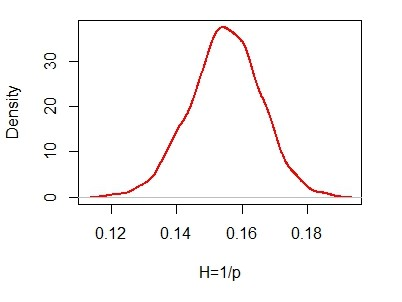
\includegraphics[width=\linewidth]{ex6_densRV.jpeg}
    \end{subfigure}
    \hfill
    \begin{subfigure}{0.48\textwidth}
        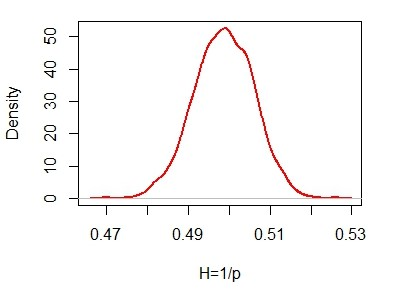
\includegraphics[width=\linewidth]{ex6_densIV.jpeg}
    \end{subfigure}
    
    \caption{Distribution of the estimated roughness index $\hat{H}_{L,K}$ via normalized $p$-th variation using $L=300\times 300$ and $K=300$ across 2500 independent simulations of the OU-SV model \eqref{eq:ousv}. \textbf{Left:} Realized volatility. \textbf{Right:} Instantaneous volatility.}
    \label{fig:ex6dens}
\end{figure}
\begin{table}[htbp]
    \centering
    \begin{tabular}{ccc}
        \toprule
         & Realized volatility & Instantaneous volatility \\
        \midrule
        Min. & 0.1192 & 0.4698 \\
        1st quartile & 0.1480 & 0.4938 \\
        Median & 0.1551 & 0.4988 \\
        Mean & 0.1549 & 0.4987 \\
        3rd quartile & 0.1621 & 0.5039 \\
        Max. & 0.1873 & 0.5257 \\
        \bottomrule
    \end{tabular}
    \caption{Summary of statistics for estimated roughness index $\hat{H}_{L,K}$ for realized and instantaneous volatility across 2500 independent simulations the OU-SV model \eqref{eq:ousv} with $L=300\times 300$ and $K=300$.}
    \label{tab:ex6dens}
\end{table}\\\\
Note that our results deviates slightly from the results in \cite{cont} for a similar model. This might be caused by \cite{cont} using the mean of $\sigma_t$ across the 300 consecutive data points as their instantaneous volatility which creates a slightly smoother volatility process. Furthermore, \cite{cont} might be using a different $T$ than us which in the OU-SV model will significantly impact the size of the estimation error and thus the estimated roughness index for realized volatility when all other parameters are kept constant. The conclusions are however the same. Realized volatility does systematically exhibit much rougher behaviour than instantaneous volatility and than the true roughness of the model. This rougher behaviour is solely caused by the estimation error, and it indicates that roughness estimated based on realized volatility can be unreliable.\\\\
In Figure \ref{fig:ex6dens} we have made density plots for the other roughness estimators across 150 independent paths generated from the OU-SV model \eqref{eq:ousv}. The left plot of Figure \ref{fig:ex6dens} displays density plots of the estimators when used on realized volatility and realized variance whereas the right plot displays density plots when using instantaneous volatility and $Y(\sigma_t)$ as input to the estimators. The density plot of the roughness estimator by log regression $\widehat{H}_R$ is represented by the red line. It provides very constant results. For instantaneous volatility it accurately estimates the true roughness of the underlying model whereas it for realized volatility systematically provides a roughness estimate near $0.09$ which is much rougher than the true roughness exponent $H=\frac{1}{2}$. Furthermore, we observe that the sequential scale estimator $\widetilde{\mathscr{R}}_n^s(S)$ systematically estimate the roughness of realized variance near $-0.5$. Consequently, we observe that $\lvert \widetilde{\mathscr{R}}_n^s\rvert$ is very accurate both when used for realized variance $\hat{Y}_t^{(n)}$ and for spot variance $Y(\sigma_t)$, and it is the only estimator in this example which accurately estimate the true roughness of the underlying model based on observations of the actual price process $S_t$.
\begin{figure}[htbp]
    \centering
    
    \begin{subfigure}{0.48\textwidth}
        \includegraphics[width=\linewidth]{ex6_densRV.png}
    \end{subfigure}
    \hfill
    \begin{subfigure}{0.48\textwidth}
        \includegraphics[width=\linewidth]{ex6_densIV.png}
    \end{subfigure}
    
    \caption{Density plots of the roughness estimators $\widehat{H}_R$ (red), $\widetilde{\mathscr{R}}_n^s$ (blue), $\widehat{\mathscr{R}}_n$ (green) and $\lvert \widetilde{\mathscr{R}}_n^s (S)\rvert$ (yellow) across 150 independent paths drawn from the OU-SV model \eqref{eq:ousv}. \textbf{Left:} Using realized volatility and realized variance as input. \textbf{Right:} Using instantaneous volatility $\sigma_t$ and $Y(\sigma_t)$ as input.}
    \label{fig:ex6dens}
\end{figure}\\\\
\subsection{A fractional Ornstein-Uhlenbeck model}
In the two previous models, instantaneous volatility follows a diffusive behaviour similar to a Brownian motion with $H=0.5$. We now consider a more general case of a stochastic volatility model where the volatility process has a general roughness index $H\in(0,1)$ generated from a fractional Brownian motion. We investigate the model for different roughness indexes and explore how this affect the estimation error and estimated roughness index. Consider the following process where the volatility is described by a fractional Ornstein-Uhlenbeck model:
\begin{align}
dS_t = S_t \sigma_t dB_t, \quad \sigma_t = \sigma_0 e^{Y_t}, \quad dY_t = -\gamma Y_t \, dt + \theta \, dB^H_t, \label{eq:fou}
\end{align}
where $S_t$ is the price process, $B_t$ is a Brownian motion, and $B_t^H$ is a fractional Brownian motions with Hurst exponent $H$. For the simulation we use the parameters $\sigma_0 =\gamma=\theta=1$ and $Y_0=0$, and we set $T=5$ and $S_0=1$.\\\\
We now repeat the procedure described in section 4.1 to compute the estimated roughness index $\hat{H}_{L,K}$ with $L=300\times 300$ and $K=300$ for realized and instantaneous volatility. Furthermore, we compute the smoothness parameter from section 3.5 for both the realized and instantaneous volatility. We compute these roughness estimates across different values of the true Hurst exponent $H$. In Table \ref{tab:ex7table} we have computed roughness estimates from the fractional Ornstein-Uhlenbeck model \eqref{eq:fou} with Hurst exponent $H=\{0.1,0.2,0.3,0.4,0.5,0.6,0.7,0.8\}$. We have used the same seed in the simulation for all values of $H$ such that the underlying stochastic element of the price processes are the same. Thus, the difference between the price processes solely lies in the Hurst exponent $H$.
\begin{table}[htbp]
    \centering
    \begin{tabular}{cccccc}
        \toprule
        H & Instantaneous vol & Realized vol & IV (log reg) & RV (log reg)\\
        \midrule
        0.1 & 0.126 & 0.199 & 0.102 & 0.197\\
        0.2 & 0.220 & 0.256 & 0.204 & 0.250\\
        0.3 & 0.313 & 0.261 & 0.305 & 0.257\\
        0.4 & 0.408 & 0.218 & 0.407 & 0.188\\
        0.5 & 0.504 & 0.159 & 0.508 & 0.095\\
        0.6 & 0.598 & 0.102 & 0.607 & 0.036\\
        0.7 & 0.691 & 0.070 & 0.703 & 0.012\\
        0.8 & 0.778 & 0.052 & 0.794 & 0.004\\
        \bottomrule
    \end{tabular}
    \caption{Estimated roughness via $p$-th variation $\hat{H}_{L,K}$ and via log regression for instantaneous and realized volatility for simulated data from a fractional Ornstein-Uhlenbeck model \eqref{eq:fou} with Hurst exponent $H=\{0.1,0.2,0.3,0.4,0.5,0.6,0.7,0.8\}$.}
    \label{tab:ex7table}
\end{table}\\\\
The corresponding paths for price process, realized volatility and instantaneous volatility from model \ref{eq:fou} with Hurst exponent $H=\{0.1,0.2,0.3,0.4,0.5,0.6,0.7,0.8\}$ are presented in Figure \ref{fig:ex7paths}. Visually we observe that the price processes do not differ much as the Hurst exponent changes. However, the paths of realized and instantaneous volatility are very different for different Hurst exponents. For small Hurst exponents instantaneous volatility does visually appear more rough than realized volatility. However, instantaneous volatility becomes smoother and smoother as $H$ increases. That is expected since increasing the Hurst exponent $H$ exactly means that the volatility process becomes smoother. However, realized volatility is not gradually getting smoother as $H$ increases. Instead we observe that for large Hurst exponents, realized volatility appears very rough. This is supported by the estimated roughness indices in Table \ref{tab:ex7table}. The estimated roughness based on instantaneous volatility is increasing as $H$ increases both for the roughness estimator via $p$-th variation and the estimator via logarithmic regression. The estimated roughness based on realized volatility is increasing at first as $H$ increases, but for large Hurst exponents the estimated roughness decreases and the estimated roughness of the volatility process is estimated to be very rough when the true Hurst exponent is $H=0.8$. 
\begin{figure}[htbp]
    \centering
    
    \begin{subfigure}{0.32\textwidth}
        \includegraphics[width=\linewidth]{H01_S.png}
    \end{subfigure}
    \hfill
    \begin{subfigure}{0.32\textwidth}
        \includegraphics[width=\linewidth]{H01_RV.png}
    \end{subfigure}
    \hfill
    \begin{subfigure}{0.32\textwidth}
        \includegraphics[width=\linewidth]{H01_IV.png}
    \end{subfigure}
    \vskip 0em
    \begin{subfigure}{0.32\textwidth}
        \includegraphics[width=\linewidth]{H02_S.png}
    \end{subfigure}
    \hfill
    \begin{subfigure}{0.32\textwidth}
        \includegraphics[width=\linewidth]{H02_RV.png}
    \end{subfigure}
    \hfill
    \begin{subfigure}{0.32\textwidth}
        \includegraphics[width=\linewidth]{H02_IV.png}
    \end{subfigure}
        \vskip 0em
    \begin{subfigure}{0.32\textwidth}
        \includegraphics[width=\linewidth]{H03_S.png}
    \end{subfigure}
    \hfill
    \begin{subfigure}{0.32\textwidth}
        \includegraphics[width=\linewidth]{H03_RV.png}
    \end{subfigure}
    \hfill
    \begin{subfigure}{0.32\textwidth}
        \includegraphics[width=\linewidth]{H03_IV.png}
    \end{subfigure}
        \vskip 0em
    \begin{subfigure}{0.32\textwidth}
        \includegraphics[width=\linewidth]{H04_S.png}
    \end{subfigure}
    \hfill
    \begin{subfigure}{0.32\textwidth}
        \includegraphics[width=\linewidth]{H04_RV.png}
    \end{subfigure}
    \hfill
    \begin{subfigure}{0.32\textwidth}
        \includegraphics[width=\linewidth]{H04_IV.png}
    \end{subfigure}
        \vskip 0em
    \begin{subfigure}{0.32\textwidth}
        \includegraphics[width=\linewidth]{H05_S.png}
    \end{subfigure}
    \hfill
    \begin{subfigure}{0.32\textwidth}
        \includegraphics[width=\linewidth]{H05_RV.png}
    \end{subfigure}
    \hfill
    \begin{subfigure}{0.32\textwidth}
        \includegraphics[width=\linewidth]{H05_IV.png}
    \end{subfigure}
        \vskip 0em
    \begin{subfigure}{0.32\textwidth}
        \includegraphics[width=\linewidth]{H06_S.png}
    \end{subfigure}
    \hfill
    \begin{subfigure}{0.32\textwidth}
        \includegraphics[width=\linewidth]{H06_RV.png}
    \end{subfigure}
    \hfill
    \begin{subfigure}{0.32\textwidth}
        \includegraphics[width=\linewidth]{H06_IV.png}
    \end{subfigure}
        \vskip 0em
    \begin{subfigure}{0.32\textwidth}
        \includegraphics[width=\linewidth]{H07_S.png}
    \end{subfigure}
    \hfill
    \begin{subfigure}{0.32\textwidth}
        \includegraphics[width=\linewidth]{H07_RV.png}
    \end{subfigure}
    \hfill
    \begin{subfigure}{0.32\textwidth}
        \includegraphics[width=\linewidth]{H07_IV.png}
    \end{subfigure}
        \vskip 0em
    \begin{subfigure}{0.32\textwidth}
        \includegraphics[width=\linewidth]{H08_S.png}
    \end{subfigure}
    \hfill
    \begin{subfigure}{0.32\textwidth}
        \includegraphics[width=\linewidth]{H08_RV.png}
    \end{subfigure}
    \hfill
    \begin{subfigure}{0.32\textwidth}
        \includegraphics[width=\linewidth]{H08_IV.png}
    \end{subfigure}
    
    \caption{ \textbf{Left:} Simulated price path $S_t-S_0$ of fractional OU model \ref{eq:fou} with Hurst exponent $H=\{0.1,0.2,0.3,0.4,0.5,0.6,0.7,0.8\}$ respectively. \textbf{Center:} Realized volatility. \textbf{Right:} Instantaneous volatility.}
    \label{fig:ex7paths}
\end{figure}\\\\
In Figure \ref{fig:ex7single} we have plotted the values from Table \ref{tab:ex7table} in a graph. The blue lines represents roughness estimates for instantaneous volatility while the red lines represents roughness estimates for the corresponding realized volatility. The solid lines are the estimated roughness index via $p$-th variation $\hat{H}_{L,K}$ with $L=300\times 300$ and $K=300$ while the dashed lines represent roughness estimates using the smoothness parameter computed by logarithmic regression. The $x$-axis represent the true value of $H$ of the simulated fractional OU model. We observe that roughness estimates based on instantaneous volatility give accurate estimates of the true Hurst index $H$. However, the estimated roughness for realized volatility is quite inaccurate and always stay below $0.3$. In particular, when the instantaneous volatility process is generated from a smooth process (i.e. $H>\frac{1}{2}$) the roughness estimate of realized volatility turns out to be a very poor estimate.\\ 
It seems that our two roughness estimates coincides and generate similar estimates. Only when the true model is smooth (i.e. $H>0.5$) the roughness estimate by logarithmic regression for realized volatility seems to systematically be rougher that the corresponding roughness estimate via $p$-th variation. However, both estimates are very poor in this case. 
\begin{figure}[htbp]
    \centering
    
    \begin{subfigure}{0.78\textwidth}
        \includegraphics[width=\linewidth]{ex7_single_plot.png}
    \end{subfigure}
    
    \caption{Estimated roughness indexes for realized and instantaneous volatility from a fractional OU model (\ref{eq:fou}) plotted for price paths generated by different values of $H$. The solid lines are roughness indexes via $p$-th variation $\hat{H}_{L,K}$ with $L = 300\times 300$ and $K= 300$ while the dashed lines represents estimated roughness by logarithmic regression.}
    \label{fig:ex7single}
\end{figure}\\\\
In Figure \ref{fig:ex7plot100} we have repeated the above analyses for 100 independent simulated prices processes generated by the fractional Ornstein-Uhlenbeck model \eqref{eq:fou} but only for the estimated roughness index via $p$-th variation $\hat{H}_{L,K}$ with $L = 100\times 100$ and $K= 100$. The figure shows the estimators $\hat{H}_{L,K}(RV)$ and $\hat{H}_{L,K}(\sigma)$ plotted against Hurst exponents $H=\{0.1,0.2,0.3,0.4,0.5,0.6,0.7,0.8\}$ for every independent path. The bold black lines represent the mean across 100 independent simulations whereas the dotted lines represent the corresponding 75\% confidence interval. If equation \eqref{eq:wpth} have no solution for $H\in (0,1)$ we set $\hat{H}_{L,K}=0$.
\begin{figure}[htbp]
    \centering
    
    \begin{subfigure}{0.78\textwidth}
        \includegraphics[width=\linewidth]{ex7_plot100.png}
    \end{subfigure}
    
    \caption{Estimated roughness index via $p$-th variation for realized and instantaneous volatility plotted against different values of $H$ for 100 independent price paths from a fractional OU model (\ref{eq:fou}). The solid black lines represent the mean across the 100 paths and the dashed black lines represent the corresponding 75\% confidence interval.}
    \label{fig:ex7plot100}
\end{figure}\\\\
From Figure \ref{fig:ex7plot100} we observe that for all 100 independent simulations the roughness estimators exhibit a similar behaviour. Our conclusions about the poorness of roughness estimates for realized volatility still hold and was not just a matter of the single price path we studied before. In particular, for the fractional Ornstein-Uhlenbeck model \eqref{eq:fou} realized volatility always exhibit rough behaviour (i.e. $H<\frac{1}{2}$) no matter what the true roughness of the volatility process is. The estimated roughness based on instantaneous volatility is quite accurate and as this is a simulation study we have no measurement errors so the inaccuracy of the estimators for realized volatility solely comes from the estimation error. \\\\
We now introduce the absolute sequential scale estimator $\lvert \widehat{\mathscr{R}}_n^s\rvert$ to this example. We take a slightly different approach than in the previous examples and simulate directly the required observations needed for the sequential scale estimator from model \eqref{eq:fou} with $T=1$. We use $n=16$ and $m_n = 2^4$ for the estimation. For the same price path we also compute the roughness index via $p$-th variation $\hat{H}_{L,K}$ and the roughness estimator via log regression $\widehat{H}_R$ by computing instantaneous and realized volatility for every 300 consecutive points. Thus, we use $L=13980$ and $K=\sqrt{L}$ for the estimator $\hat{H}_{L,K}$. In Table \ref{tab:ex7tableincl_scale} we display the roughness estimates obtained for Hurts exponent $H=\{0.1,.0.2,0.3,0.4,0.5,0.6,0.7,0.8\}$. We have used the same seed for all $H$ values. The estimates from $\lvert \widehat{\mathscr{R}}_n^s\rvert$ are displayed in the two columns furthest to the right in Table \ref{tab:ex7tableincl_scale}. IV should for this estimator be understood as integrated variance approximated directly from instantaneous volatility as in \eqref{eq:ex5y} whereas RV should be understood as realized variance computed as in \eqref{eq:rvforscale}. For $\widehat{H}_{L,K}$ and $\widehat{H}_{R}$ we obtain similar results to the estimates from Table \ref{tab:ex7table} and both of these estimates are inaccurate when used for realized volatility and always stay below 0.3. However, the absolute scale estimator $\lvert \widehat{\mathscr{R}}_n^s\rvert$ performs differently. We observe that the estimator is accurate when using spot variance $Y(\sigma_t)$ as input. When using realized variance as input the estimator is not very accurate, but it performs better than the other two roughness estimators, and it does not estimate the process to be rough (i.e. $H<\frac{1}{2}$) when the true underlying model is actually smooth (i.e. $H>\frac{1}{2}$).
\begin{table}[htbp]
    \centering
    \begin{tabular}{cccccccc}
        \toprule
        H & IV ($\widehat{H}_{L,K}$) & RV ($\widehat{H}_{L,K}$) & IV ($\widehat{H}_{R}$) & RV ($\widehat{H}_{R}$) & IV ($\lvert \widehat{\mathscr{R}}_n^s\rvert$) & RV ($\lvert \widehat{\mathscr{R}}_n^s\rvert$)\\
        \midrule
        0.1 & 0.140 & 0.226 & 0.102 & 0.192 & 0.067 & 0.175\\
        0.2 & 0.219 & 0.275 & 0.202 & 0.246 & 0.189 & 0.294\\
        0.3 & 0.312 & 0.275 & 0.300 & 0.259 & 0.294 & 0.445\\
        0.4 & 0.408 & 0.216 & 0.399 & 0.201 & 0.396 & 0.501\\
        0.5 & 0.503 & 0.150 & 0.498 & 0.109 & 0.498 & 0.510\\
        0.6 & 0.593 & 0.107 & 0.596 & 0.044 & 0.599 & 0.510\\
        0.7 & 0.676 & 0.077 & 0.691 & 0.016 & 0.699 & 0.509\\
        0.8 & 0.749 & 0.055 & 0.780 & 0.005 & 0.799 & 0.508\\
        \bottomrule
    \end{tabular}
    \caption{Estimated roughness for the three roughness estimators $\widehat{H}_{L,K}$, $\widehat{H}_R$ and $\lvert \widehat{\mathscr{R}}_n^s\rvert$ using instantaneous volatility (IV) and realized volatility/variance (RV) for simulated data from a fractional Ornstein-Uhlenbeck model \eqref{eq:fou} with Hurst exponent $H=\{0.1,0.2,0.3,0.4,0.5,0.6,0.7,0.8\}$.}
    \label{tab:ex7tableincl_scale}
\end{table}\\\\
In the left plot of Figure \ref{fig:ex7singleincl_scale} we have plotted the results from Table \ref{tab:ex7tableincl_scale} to visualize the estimates. The right plot of Figure \ref{fig:ex7singleincl_scale} shows roughness estimates from the absolute scale estimator $\lvert \widehat{\mathscr{R}}_n^s\rvert$ across 100 independent price paths plotted against the true roughness of the model $H=\{0.1,0.2,0.3,0.4,0.5,0.6,0.7,0.8\}$. Thus, it is 100 repetitions of the procedure described above. The bold black lines represent the mean acroos 100 independent simulations whereas the dotted lines represent a 75\% confidence interval. 
\begin{figure}[htbp]
    \centering
    
    \begin{subfigure}{0.48\textwidth}
        \includegraphics[width=\linewidth]{ex7_single_all.png}
    \end{subfigure}
    \hfill
    \begin{subfigure}{0.48\textwidth}
        \includegraphics[width=\linewidth]{ex7_final100scale.png}
    \end{subfigure}
    
    \caption{Estimated roughness indexes using instantaneous volatility (IV) and realized volatility/variance (RV) from a fractional OU model (\ref{eq:fou}) with $T=1$ plotted for price paths generated by different values of $H$. \textbf{Left:} Estimates for all three roughness estimators $\widehat{H}_{L,K}$, $\widehat{H}_R$ and $\lvert \widehat{\mathscr{R}}_n^s\rvert$ . \textbf{Right:} Absolute scale estimates $\lvert \widehat{\mathscr{R}}_n^s\rvert$ for 100 independent price paths. The solid black line represents the mean, and the dashed black lines represent a 75\% confidence interval.}
    \label{fig:ex7singleincl_scale}
\end{figure}\\\\
From Figure \ref{fig:ex7singleincl_scale} we conclude that the absolute scale estimator systematically exhibits the same kind of behaviour. That is, when used for realized variance the estimator is not very precise especially when the true roughness exponent of the underlying model takes a high value. However, it does remedy some of the inaccuracies observed for the other two estimators, and it does not estimate the path to be rough when the underlying model is not rough. As this is a simulation study, the difference between the blue and red lines are solely caused by estimation errors. \\\\
In practice, instantaneous volatility cannot be observed, and roughness estimates are based on realized volatility. If using traditional roughness estimators such as $\widehat{H}_{L,K}$ and $\widehat{H}_R$, the above examples illustrate that one cannot necessarily draw the conclusion that (spot) volatility is rough just because realized volatility exhibit rough behaviour with $\hat{H}_{L,K}(RV)<\frac{1}{2}$ even if the estimated roughness is well below $\frac{1}{2}$.\\
Passing to the absolute sequential scale estimator $\lvert \widehat{\mathscr{R}}_n^s\rvert$ which is developed with the ambition of accurately estimating roughness from realized variance does in these examples improve estimation from realized input. However, $\lvert \widehat{\mathscr{R}}_n^s\rvert$ is also somewhat vulnerable to estimation errors and does not completely remove inaccuracies caused by estimation errors. Furthermore, $\lvert \widehat{\mathscr{R}}_n^s\rvert$ requires observations of realized variance for very specific time points making it less applicable to real time high frequency data. 

\subsection{RFSV model}
We will now consider the stochastic volatility model suggested by \cite{gatheral}. The model is defined in the following way:
\begin{align}
dS_t = S_t \sigma_t \sqrt{dt}U_n, \quad \sigma_t = e^{Y_t}, \quad dY_t = -\alpha (Y_t-m) \, dt + \nu \, dB^H_t, \label{eq:rfsv}
\end{align}
for some $\nu>0$, $\alpha>0$, $m\in\mathbb{R}$ and $H<\frac{1}{2}$ where $B^H_t$ is a fractional Brownian motion and $U_n$ are iid standard Gaussian variables. \cite{gatheral} further argues that choosing $\alpha \ll \frac{1}{T}$ is desirable since the log-volatility then locally behaves like a fBm while it is still technically stationary. In addition to this, \cite{gatheral} argues that observed skew term structure in financial data can easier be replicated by choosing $\alpha \ll \frac{1}{T}$.\\\\
The specified RFSV model is similar to model (\ref{eq:fou}) from section 4.3 and both models use a fractional Ornstein-Uhlenbeck process to model log-volatility. In this section we use a different approach to compute realized and instantaneous volatility. We follow much of the simulation approach from \cite{gatheral}. We set $T=3601$ and simulate 5000 point per day. For every day we compute the realized volatility of the first 1000 points of the day, and we then rescale this volatility to be a daily volatility estimate. The corresponding instantaneous volatility is computed as the mean of the first 1000 points per day. Following this approach to compute volatility data, we perform many of the same analyses as in section 4.3. When simulating from the model we use the parameters $\nu = 0.2$, $\alpha = 10^{-4}$, $m = -7$ and we set $Y_0=m$ and $S_0 = 1$.\\\\
In Table \ref{tab:ex8table} we have computed roughness estimates from the RSFV model (\ref{eq:rfsv}) with Hurst exponent $H= \{0.1,0.2,0.3,0.4,0.5\}$.
\begin{table}[htbp]
    \centering
    \begin{tabular}{cccccc}
        \toprule
        H & Instantaneous vol & Realized vol & IV (log reg) & RV (log reg)\\
        \midrule
        0.1 & 0.175 & 0.168 & 0.146 & 0.143\\
        0.2 & 0.241 & 0.236 & 0.217 & 0.214\\
        0.3 & 0.314 & 0.310 & 0.297 & 0.295\\
        0.4 & 0.394 & 0.390 & 0.386 & 0.384\\
        0.5 & 0.475 & 0.472 & 0.478 & 0.476\\
        \bottomrule
    \end{tabular}
    \caption{Estimated roughness via $p$-th variation $\hat{H}_{L,K}$ with $L=60\times60$ and $K=60$ and via log regression for instantaneous and realized volatility for simulated data from the RSFV model \eqref{eq:rfsv} with Hurst exponent $H=\{0.1,0.2,0.3,0.4,0.5\}$.}
    \label{tab:ex8table}
\end{table}
\begin{figure}[htbp]
    \centering
    
    \begin{subfigure}{0.78\textwidth}
        \includegraphics[width=\linewidth]{rsfv_single.jpeg}
    \end{subfigure}
    
    \caption{Estimated roughness indexes for realized and instantaneous volatility from a RSFV model (\ref{eq:fou}) plotted for price paths generated by different values of $H$. The solid lines are roughness indexes via $p$-th variation $\hat{H}_{L,K}$ with $L = 3600$ and $K= 60$ while the dashed lines represents estimated roughness by logarithmic regression.}
    \label{fig:rsfv_single}
\end{figure}\\\\

\section{Conclusion}
In this thesis we have investigated roughness of volatility processes in financial time series and taken a closer look at the claim 'volatility is rough'. More precisely, we have investigated the robustness of roughness estimates based on realized volatility for three different roughness estimators. Most roughness estimators in literature rely on approximating true spot volatility $\sigma_t$ by realized volatility and then estimating the roughness of these proxy values $\hat{\sigma}_t$. We introduce two roughness estimators based on this approach, the roughness estimator via normalized $p$-th variation statistics $\widehat{H}_{L,K}$ and the roughness estimator by logarithmic regression $\widehat{H}_R$. We have in this thesis shown that such estimates based on realized volatility can be unreliable. We have conducted numerical experiments, and as described in section 4.1 and 4.2 we find that for two stochastic volatility diffusion models driven by a Brownian motion, realized volatility exhibit rough behaviour with an estimated roughness index significantly smaller than the true roughness index $H=\frac{1}{2}$. For our two stochastic diffusive examples we estimate the roughness of realized volatility in the range $\widehat{H}\approx 0.3$ and $\widehat{H}\approx 0.15$ respectively. However, when estimating directly from instantaneous volatility we obtain accurate results very close to the true roughness of the underlying model $H=\frac{1}{2}$. The two estimators $\widehat{H}_{L,K}$ and $\widehat{H}_R$ widely coincides, and generate very similar results in all cases. As these are simulation examples, this apparent rough behaviour of realized volatility is entirely caused by the difference between realized volatility and instantaneous volatility also known as the estimation error. These results suggest that it cannot necessarily be concluded that observed rough behaviour in realized volatility is an indicator of similar behaviour in true spot volatility.\\\\
Moreover, we show in section 4.3 and 4.4 that for volatility processes driven by a fractional Ornstein-Uhlenbeck model, realized volatility always exhibit rough behaviour (i.e. $\widehat{H}<\frac{1}{2}$). For both of these examples even when the true underlying model has diffusive or smooth behaviour (i.e. $H\geq \frac{1}{2}$) the roughness estimates based on realized volatility always stay below $0.3$. If we estimate roughness directly from instantaneous volatility we obtain accurate estimates, and this again indicates that the estimation error can substantially distort the outcome of the roughness estimation. More precisely, these results show that stochastic diffusive models or even smooth volatility processes are perfectly compatible with rough behaviour observed in realized volatility. The conclusions from 'rough volatility' literature such as \cite{gatheral} stating that 'volatility is rough' because \\\\
In this thesis we also introduce a third roughness estimator, the sequential scale estimator $\widehat{\mathscr{R}}_n^s$ first introduced by \cite{han}. This estimator estimates the roughness of a path from discrete observations of integrated variance or realized variance and is developed with the purpose of minimizing the possible distortion caused by estimation errors. We find that by modifying the estimator into the absolute sequential scale estimator $\lvert \widehat{\mathscr{R}}_n^s \rvert$ we do obtain more accurate estimates from realized data compared to our other two roughness estimators. For our two stochastic diffusive models in section 4.1 and 4.2, $\lvert \widehat{\mathscr{R}}_n^s \rvert$ performs very well when using realized variance as input, and it accurately estimates the true roughness of the underlying model $H=\frac{1}{2}$. Thus, in these two examples $\lvert \widehat{\mathscr{R}}_n^s \rvert$ completely remedies the apparent rough behaviour of realized volatility. However, for our models driven by a fractional Ornstein-Uhlenbeck model in section 4.3 and 4.4, the absolute sequential scale estimator does not perform as well as before. Here we find that $\lvert \widehat{\mathscr{R}}_n^s \rvert$ tends to always estimate the roughness of realized variance near $0.5$ when the underlying model is actually smooth (i.e. $H>\frac{1}{2}$). When the underlying model is rough (i.e. $H<\frac{1}{2}$) $\lvert \widehat{\mathscr{R}}_n^s \rvert$ tends to overestimate the true roughness such that it in all cases estimates the path to be nearer to diffusive behaviour (i.e. $H=\frac{1}{2}$) than the true model actually is. \\
When we instead of realized variance use integrated variance computed directly from instantaneous volatility $\sigma_t$ as input, the sequential scale estimator performs very well, and does in all cases estimate the true roughness of the model accurately. Thus, $\lvert \widehat{\mathscr{R}}_n^s \rvert$ is also vulnerable to estimation errors where estimation error in this case means the difference between realized variance and integrated variance. \\\\
Comparing our three roughness estimators we find that they all perform very well in our examples when based on instantaneous volatility. $\widehat{H}_{L,K}$ and $\lvert \widehat{\mathscr{R}}_n^s \rvert$ work in a model-free setting and are therefore very flexible and applicable to many different models. Estimators like $\widehat{H}_R$ only works well if the class of models is well-specified. However, $\widehat{H}_R$ seems to converge faster, and it requires less data input for the estimate to be accurate.\\
For realized volatility/variance $\lvert \widehat{\mathscr{R}}_n^s \rvert$ does in some cases perform much better than the other two estimators, but it does not estimate the roughness of the underlying model accurately in all cases. Furthermore, $\lvert \widehat{\mathscr{R}}_n^s \rvert$ has much stronger requirements to the input data, and it needs observations at very specific time points. That makes the estimator less applicable to real world high-frequency data where the discrete grid of observation times might not be a uniform partition sequence.\\\\
For future investigation it could be relevant to investigate how the absolute sequential scale estimator $\lvert \widehat{\mathscr{R}}_n^s \rvert$ could be further improved. The estimation error for this estimator is as shown very small, and if the estimator could fully handle this estimation error it has the potential to perform reliable roughness estimates from realized data. Another thing that could be further investigated is the estimation error itself. If it turns out that the estimation error is insignificant when using a certain approach to calculate it or a certain set of models, it would shed light on when to expect reliable roughness estimates. Both of these things could be a helping tool in determining whether volatility is rough or not.

\newpage
\section{Appendix}
\subsection{Simulation of fractional Brownian motion} \label{sec:sim_fbm}
Throughout this thesis we will be simulating from the fractional Brownian motion by using a spectral method which can be used for stationary processes. The idea is to analyse the stochastic process in the spectral domain rather than the time domain. The spectral density is computed as follows for frequencies $-\pi\leq \lambda \leq \pi$:
\begin{align}
f(\lambda):= \sum_{j=-\infty}^\infty \gamma(j) \exp(ij\lambda)
\end{align}
where $\gamma(\cdot)$ represent the autocovariance function. It can be shown that the spectral density of fractional Gaussian noise is given by
\begin{align}
f(\lambda) = 2\sin(\pi H)\Gamma(2H+1)(1-\cos\lambda)[\vert\lambda\vert ^{-2H-1}+B(\lambda, H)]
\end{align}
where $\Gamma(\cdot)$ denotes the Gamma function and 
\begin{align}
B(\lambda, H) := \sum_{j=1}^\infty \left((2\pi j+\lambda)^{-2H-1}+(2\pi j-\lambda)^{-2H-1}\right)
\end{align}
for $-\pi\leq \lambda \leq \pi$. The infinite sum makes direct numerical evaluation almost impossible. However, a useful approximation of the sum is made by \cite{paxson}. They show that by using
\begin{align*}
&\tilde{B}_3(\lambda, H) :=\\ 
&\sum_{j=1}^3 \left(\left(a_j^+\right)^{-2H-1}+\left(a_j^-\right)^{-2H-1}\right)+\frac{\left(a_3^+\right)^{-2H}+\left(a_3^-\right)^{-2H}+\left(a_4^+\right)^{-2H}+\left(a_4^-\right)^{-2H}}{8H\pi}
\end{align*}
where $a^{\pm}_j=2\pi j\pm \lambda$, $f(\lambda)$ is approximated quite well.\\\\
Now, consider a stationary Gaussian discrete-time process $X=\{X_n: n = 0,...,N-1\}$ where $N$ is the required sample size. The spectral theorem states that it can be represented in terms of the spectral density as
\begin{align}
X_n\overset{d}{=}\int_0^\pi \sqrt{\frac{f(\lambda)}{\pi}}\cos(n\lambda)dB_1(\lambda)-\int_0^\pi \sqrt{\frac{f(\lambda)}{\pi}}\sin(n\lambda)dB_2(\lambda)
\end{align}
where $B_1$ and $B_2$ are two mutually independent Brownian motions \cite{dieker}. We wish to approximate (8). The integrand is replaced by a simpler function. Fix some integer $l$ and set $t_k = \pi k/l$ for $k=0,...,l$. Now, define a simple function $\xi_n^{(l)}$ on $[0,\pi]$ for $0\leq n\leq N-1$ by 
\begin{align}
\xi_n^{(\ell)}(\lambda)= \sqrt{\frac{f(t_1)}{\pi}}\cos(nt_1)\mathbf{1}_{\{0\}}(\lambda)+\sum_{k=0}^{l-1} \sqrt{\frac{f(t_{k+1})}{\pi}}\cos(nt_{k+1})\mathbf{1}_{(t_k,t_{k+1}]}(\lambda).
\end{align}
The first integral in $(8)$ can be approximated by $\int_0^\pi \xi_n^{(\ell)}(\lambda)dB_1(\lambda)$. Since $\xi_n^{(\ell)}$ is a simple function the stochastic integral can be computed as
\begin{align}
\int_0^\pi \xi_n^{(l)}(\lambda)dB_1(\lambda) = \sum _{j=0}^{\ell-1} \xi_n^{(l)} (B(t_{j+1})-B(t_j)).
\end{align} 
Thus, we obtain 
\begin{align*}
&\int_0^\pi \xi_n^{(l)}(\lambda)dB_1(\lambda) = \sum_{j=0}^{\ell-1}\sum_{k=0}^{\ell-1} \sqrt{\frac{f(t_{k+1})}{\pi}} \cos(n t_{k+1}) \mathbf{1}_{(t_k,t_{k+1}]}(B_1(t_{j+1})-B_1(t_j))\\
&= \sum_{k=0}^{l-1} \sqrt{\frac{f(t_{k+1})}{\pi}} \cos(n t_{k+1}) 
(B_1(t_{k+1})-B_1(t_k)) \\
&= \sum_{k=0}^{\ell-1} \sqrt{\frac{f(t_{k+1})}{\pi}} \cos(n t_{k+1})U_k^{(0)} \sqrt{\frac{\pi}{l}} = \sum_{k=0}^{\ell-1} \sqrt{\frac{f(t_{k+1})}{\ell}} \cos(n t_{k+1})U_k^{(0)} \label{eq:sim_xn}
\end{align*}
where $U_k^{(0)}$ is an i.i.d. standard normal random variable for $k=0,...,\ell-1$. The $U_k^{(0)}\sqrt{\pi/\ell}$ represent the Brownian motion increments which per definition are normally distributed with mean $0$ and variance $t_{k+1}-t_k$.\\\\
The second integral in $(8)$ can be approximated in a similar way by replacing the cosine terms with sine terms. Thus, we obtain the following approximation of $X_n$:
\begin{align}
\hat{X}_n^{(\ell)} := \sum_{k=0}^{\ell-1} \sqrt{\frac{f(t_{k+1})}{\ell}}\left( \cos(nt_{k+1})U_k^{(0)}-\sin (nt_{k+1}) U_k^{(1)}\right).
\end{align}
The two vectors $U^{(0)}$ and $U^{(1)}$ are mutually independent since $B_1$ and $B_2$ are independent as well. In order to calculate $\hat{X}_n^{(\ell)}$ efficiently we will be using the fast Fourier transform (FFT). To this end, we define the sequence $(a_k)_{k=0,...,2\ell-1}$ by

\[
a_k := \begin{cases}
0 & k = 0; \\
\frac{1}{2} \left( U^{(0)}_{k-1} + i U^{(1)}_{k-1} \right) \sqrt{\frac{f(t_k)}{\ell}} & k = 1, \dots, \ell - 1; \\
U^{(0)}_{k-1} \sqrt{\frac{f(t_k)}{\ell}} & k = \ell; \\
\frac{1}{2} \left( U^{(0)}_{2\ell - k - 1} - i U^{(1)}_{2\ell - k - 1} \right) \sqrt{\frac{f(t_{2\ell - k})}{\ell}} & k = \ell + 1, \dots, 2\ell - 1.
\end{cases}
\]
It is shown in Appendix \ref{sec:sim_proof} that the Fourier transform of $a_k$ is indeed real and equals $\hat{X}_n^{(\ell)}$. From this approximated fractional Gaussian noise we can generate the fBm. \\\\
\cite{dieker} shows that the finite-dimensional distributions of $\hat{X}^{(\ell)}$ converge in probability to the corresponding finite-dimensional distributions of $X$ as $\ell\rightarrow \infty$. The rate of convergence is, however, quite slow. Therefore, we will be using a $\ell \geq 30000$ when simulating from the fBm by the spectral method in this thesis in order to make sure that our simulations are reliable. Figure \ref{fig:fbmsim} shows three simulations of fractional Brownian motions with different Hurst parameters generated by the spectral method. 
\begin{figure}[h]
    \centering
    \begin{subfigure}{0.32\textwidth}
        \centering
        \includegraphics[width=\textwidth]{specsim1.jpeg}
        \caption{H=0.2}
    \end{subfigure}\hfill
    \begin{subfigure}{0.32\textwidth}
        \centering
        \includegraphics[width=\textwidth]{specsim2.jpeg}
        \caption{H=0.5}
    \end{subfigure}\hfill
    \begin{subfigure}{0.32\textwidth}
        \centering
        \includegraphics[width=\textwidth]{specsim3.jpeg}
        \caption{H=0.8}
    \end{subfigure}
    \caption{Fractional Brownian motions generated by the spectral method.}
    \label{fig:fbmsim}
\end{figure}
\subsubsection{Proof of Fourier transform in spectral method} \label{sec:sim_proof}
Consider 
\[
a_k := \begin{cases}
0 & k = 0; \\
\frac{1}{2} \left( U^{(0)}_{k-1} + i U^{(1)}_{k-1} \right) \sqrt{\frac{f(t_k)}{\ell}} & k = 1, \dots, \ell - 1; \\
U^{(0)}_{k-1} \sqrt{\frac{f(t_k)}{\ell}} & k = \ell; \\
\frac{1}{2} \left( U^{(0)}_{2\ell - k - 1} - i U^{(1)}_{2\ell - k - 1} \right) \sqrt{\frac{f(t_{2\ell - k})}{\ell}} & k = \ell + 1, \dots, 2\ell - 1.
\end{cases}
\]
We want to take the Fourier transform of this sequence. The Fourier transform of $(a_k)_{k=0}^{2\ell-1}$ is $\lambda_n = \sum_{k=0}^{2\ell-1} a_k \exp(2\pi i \frac{nk}{2\ell})$. By Euler's formula we obtain
\begin{align*}
\lambda_n = \sum_{k=0}^{2\ell-1} a_k \left( \cos\left(\pi\frac{nk}{\ell}\right) + i\sin\left(\pi \frac{nk}{\ell}\right)\right).
\end{align*}
We will now insert $a_k$ and split the sum into the four different cases of $a_k$. Hence, we obtain
\begin{align*}
&\lambda_n = 0 + \sum_{k=1}^{l-1} \frac{1}{2} \left( U^{(0)}_{k-1} + i U^{(1)}_{k-1} \right) \sqrt{\frac{f(t_k)}{\ell}} \left( \cos\left(\pi\frac{nk}{\ell}\right) + i\sin\left(\pi \frac{nk}{\ell}\right)\right)\\
&+ U^{(0)}_{\ell-1} \sqrt{\frac{f(t_\ell)}{\ell}}\left( \cos\left(\pi\frac{n\ell}{\ell}\right) + i\sin\left(\pi \frac{n\ell}{\ell}\right)\right)\\
&+ \sum_{k=l+1}^{2l-1} \frac{1}{2} \left( U^{(0)}_{2\ell - k - 1} - i U^{(1)}_{2\ell - k - 1} \right) \sqrt{\frac{f(t_{2\ell - k})}{\ell}}\left( \cos\left(\pi\frac{nk}{\ell}\right) + i\sin\left(\pi \frac{nk}{\ell}\right)\right).
\end{align*}
By definition $t_k=\frac{\pi k}{\ell}$. Thus, what is inside the cosine and sine functions is simply $nt_k$. Note that for $k=\ell$ we have $t_k=\pi$. Thus, $\sin(nt_\ell)=0$ since $n$ is an integer. By inserting this and changing the indexes of the two sums, we obtain
\begin{align*}
&\lambda_n = U^{(0)}_{\ell-1} \sqrt{\frac{f(t_\ell)}{\ell}}\cos(nt_\ell)\\
& + \sum_{k=0}^{l-2} \frac{1}{2} \left( U^{(0)}_{k}+ i U^{(1)}_{k} \right) \sqrt{\frac{f(t_{k+1})}{\ell}} \left( \cos\left(n t_{k+1}\right) + i\sin\left(n t_{k+1}\right)\right)\\
&+ \sum_{k=0}^{l-2}\frac{1}{2} \left( U^{(0)}_{\ell-k-2}- i U^{(1)}_{\ell-k-2} \right) \sqrt{\frac{f(t_{\ell-k-1})}{\ell}} \left( \cos\left(n t_{\ell+k+1}\right) + i\sin\left(n t_{\ell+k+1}\right)\right).
\end{align*}
Now note that $\sin\left(n t_{\ell+k+1}\right) = -\sin(nt_{\ell-(k+1)})$ since $t_\ell = \pi$. Similarly, $\cos\left(n t_{\ell+k+1}\right) = \cos(nt_{\ell-(k+1)})$. By inserting that in the last sum in the above expression, the sum becomes
\begin{align*}
&\sum_{k=0}^{l-2}\frac{1}{2} \left( U^{(0)}_{\ell-k-2}- i U^{(1)}_{\ell-k-2} \right) \sqrt{\frac{f(t_{\ell-k-1})}{\ell}} \left( \cos\left(n t_{\ell-k-1}\right) - i\sin\left(n t_{\ell-k-1}\right)\right)\\
& =\sum_{k=0}^{l-2}\frac{1}{2} \left( U^{(0)}_{k}- i U^{(1)}_{k} \right) \sqrt{\frac{f(t_{k+1})}{\ell}} \left( \cos\left(n t_{k+1}\right) - i\sin\left(n t_{k+1}\right)\right)
\end{align*}
where we have reversed the sum order. Now we can combine the two sums into one. Several terms cancel out such that we obtain
\begin{align*}
&\lambda_n = U^{(0)}_{\ell-1} \sqrt{\frac{f(t_\ell)}{\ell}}\cos(nt_\ell)+ \sqrt{\frac{f(t_{k+1})}{\ell}} \sum_{k=0}^{l-2} \left(U^{(0)}_k\cos\left(n t_{k+1}\right)-U^{(1)}_{k}\sin\left(n t_{k+1}\right)\right)\\
& = \sum_{k=0}^{l-1}\sqrt{\frac{f(t_{k+1})}{\ell}}\left(U^{(0)}_k\cos\left(n t_{k+1}\right)-U^{(1)}_{k}\sin\left(n t_{k+1}\right)\right)
\end{align*}
which equals the definition of $\hat{X}_n^{(\ell)}$ from \eqref{eq:sim_xn} as desired.

\newpage
\addcontentsline{toc}{section}{References}
\bibliographystyle{plainnat}
\setcitestyle{round}
\bibliography{masterRef}
\end{document}